\documentclass{article}
\overfullrule=5pt % mark overfull boxes with black TODO: should remove before handing in

\usepackage{fullpage} % decrease page margins
\usepackage[parfill]{parskip} % change new paragraph indent to new line

\usepackage{tikz} % for drawing
\usetikzlibrary{external} % cache figures to reduce compilation times
\tikzexternalize[prefix=figurecache/] % cache figures into ./figurecache/ (WARNING: directory must exist and pdflatex must be run with --shell-escape)
\usepackage{pgfplotstable}

\usepackage[labelfont=bf]{caption} % for captions
\usepackage{ifthen} % for if/else statements (in plots)

\usepackage{xargs}

\usepackage[block=space,language=australian]{biblatex}
%\DeclareFieldFormat{url}{\url{#1}} % drop URL prefix
\DeclareFieldFormat{urldate}{(visted #1)}
\addbibresource{bib.bib}
%\urlstyle{sf}
\renewcommand{\UrlFont}{\footnotesize\ttfamily}

\usepackage{siunitx}

\usepackage{amsmath}
\usepackage{commath}
\usepackage{todonotes}

\usepackage{amsthm}
\theoremstyle{definition}

\usepackage{hyperref}

\usepackage[sort,noabbrev]{cleveref} % for nicer equation references

\usepackage{xcolor}

\usepackage{pgfplots} % for plotting
\pgfplotsset{compat=1.17}
\usepgfplotslibrary{groupplots}
\usepgfplotslibrary{dateplot}

\newcommand{\Oh}{\mathcal{O}} % Fight me.

\newcommand{\Ltwoerror}[1]{\Vert #1 \Vert_2}

\newcommand\integral[4]{\int_{#3}^{#4} \dif {#2} \, {#1}}
\newcommand\integraltwo[7]{\int_{#4}^{#5} \dif {#2} \int_{#6}^{#7} \dif {#3} \, {#1}}
\usepackage{subcaption}

\usepackage{listings}
\lstset{%
  breaklines=true,
  breakatwhitespace=true,
}

%% \pgfplotsset{compat=newest,
%%     width=6cm,
%%     height=3cm,
%%     scale only axis=true,
%%     max space between ticks=25pt,
%%     try min ticks=5,
%%     every axis/.style={
%%         axis y line=left,
%%         axis x line=bottom,
%%         axis line style={thick,->,>=latex, shorten >=-.4cm}
%%     },
%%     every axis plot/.append style={thick},
%%     tick style={black, thick}
%% }
%% \tikzset{
%%     semithick/.style={line width=0.8pt},
%% }

\title{Semester Project in TMA4212}
\author{
  Thorvald M. Ballestad\\
  Jonas Bueie\\
  Knut Andre Grytting Prestsveen\\
  Herman Sletmoen
}

\begin{document}
\maketitle
\tableofcontents
\newpage

\section{Poisson equation in one dimension}
\label{task_1}

In this section, we will solve the one-dimensional Poisson equation
\begin{equation}
u_{xx} = f(x) \qquad (0 < x < 1)
\label{poisson_equation}
\end{equation}
subject to a source term $f(x)$ and different boundary conditions at $x = 0$ and $x = 1$.
First, we will solve it with finite difference methods of first and second order on a uniform grid.
Finally, we solve it on a non-uniform grid and investigate how adaptive mesh refinement (AMR) can be used to obtain accurate solutions by distributing fewer points more cleverly along the grid.

\subsection{Analytical solution}

One way to express the analytical solution is to simply integrate \cref{poisson_equation} twice to get
\begin{equation}
\begin{split}
u(x) &= C_1 + \int^x \dif x' u_x(x') \\
     &= C_1 + \int^x \dif x' \left(C_2 + \int^{x'} \dif x'' u_{xx}(x'')\right) \\
     &= C_1 + C_2 x + \int^x \dif x' \int^{x'} \dif x'' f(x''),
\label{poisson_analytical_solution}
\end{split}
\end{equation}
where the constants $C_1$ and $C_2$ are determined from two boundary conditions and the integrals can be done from any lower limit.
Note that this is equivalent to saying that the solution is a sum of the solution to the homogenuous equation $u_{xx} = 0$ and a solution to the inhomogenuous equation $u_{xx} = f(x)$.

Note that if \emph{two} Neumann boundary conditions $u_x(0) = a$ and $u_x(1) = b$ are imposed, then the solution $u(x)$ is unique only up to a constant.
If $u(x)$ is a solution to the boundary value problem defined by \cref{poisson_equation} and $u_x(0) = a$ subject to $u_x(1) = b$, then also $(u+C)_{xx} = u_{xx}$ in the interior and $(u+C)_x(0) = u_x(0) = a$ on the left boundary, and similarly on the right boundary $x=1$.
It can also be seen by observing that $C_1$ is undetermined when \ref{poisson_analytical_solution} is differentiated.

\subsection{Numerical solution on a uniform grid}

First, consider the boundary value problem defined by \cref{poisson_equation}, subject to the boundary conditions
\begin{equation*}
u(0) = a \quad \text{or} \quad u_x(0) = a \qquad \text{and} \qquad u(0) = b \quad \text{or} \quad u_x(1) = b.
\end{equation*}
To solve the equation numerically, we divide the interval $[0, 1]$ into the uniform grid 
\begin{center}
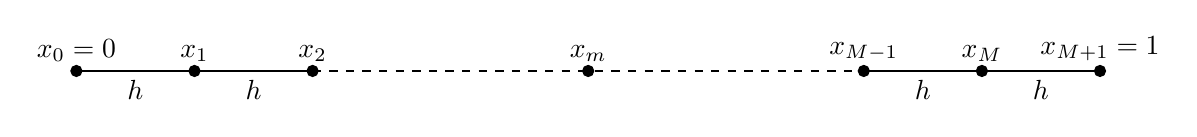
\begin{tikzpicture}
\draw (0,0) -- (3,0);
\draw[dashed] (3,0) -- (10,0);
\draw (10,0) -- (13,0);
\filldraw (0.0,0) circle (2pt) node[anchor=south] {$x_0 = 0$};
\filldraw (1.5,0) circle (2pt) node[anchor=south] {$x_1$};
\filldraw (3.0,0) circle (2pt) node[anchor=south] {$x_2$};
\filldraw (6.5,0) circle (2pt) node[anchor=south] {$x_m$};
\filldraw (10.0,0) circle (2pt) node[anchor=south] {$x_{M-1}$};
\filldraw (11.5,0) circle (2pt) node[anchor=south] {$x_{M}$};
\filldraw (13.0,0) circle (2pt) node[anchor=south] {$x_{M+1} = 1$};
\node[anchor=north] at (0.75, 0) {$h$};
\node[anchor=north] at (2.25, 0) {$h$};
\node[anchor=north] at (10.75, 0) {$h$};
\node[anchor=north] at (12.25, 0) {$h$};
\end{tikzpicture}
\end{center}
of $M+2$ points and step length $h$.
We approximate the second derivative at interior points with the central difference
\begin{equation*}
\pd{u}{x}(x_m) = \frac{u_{m-1}-2u_{m}+u_{m+1}}{h^2} + \Oh(h^2) \qquad (1 \leq m \leq M-1).
\end{equation*}
To handle the Dirichlet boundary condition $u(0) = a$ at the left edge or $u(1) = b$ at the right edge, we insert the trivial equation
\begin{equation*}
1 \cdot u_0 = a \qquad \text{or} \qquad 1 \cdot u_{M+1} = b.
\end{equation*}
To handle the Neumann boundary condition $u_x(0) = a$ at the left edge or $u_x(1) = b$ at the right edge to second order, we approximate the first derivative to second order with forward or backward differences to get
\begin{equation*}
u_x(0) = \frac{-\frac{3}{2}u_{0}-2u_1-\frac{1}{2}u_{2}}{h} + \Oh(h^2) = b \qquad \text{or} \qquad u_x(1) = \frac{\frac{1}{2}u_{M-1}-2u_M+\frac{3}{2}u_{M+1}}{h} + \Oh(h^2) = b.
\end{equation*}
Writing all these equations in $(M+2) \times (M+2)$-matrix form $AU=b$, we obtain for example with $u(0) = a$ and $u_x(1) = b$
\begin{equation}
\renewcommand{\arraystretch}{1.5} % stretch matrix vertically to make it square
\begin{bmatrix}
1 \\
+1/h^2 & -2/h^2 & +1/h^2 &   \\
  & \ddots & \ddots & \ddots & \\
  &   & +1/h^2 & -2/h^2 & +1/h^2 \\
  &   & +1/2h & -2/h & +3/2h \\
\end{bmatrix}
\begin{bmatrix}
U_0 \\ U_1 \\ \vdots \\ U_M \\ U_{M+1} \\
\end{bmatrix}
=
\begin{bmatrix}
a \\ f(x_1) \\ \vdots \\ f(x_M) \\ b \\
\end{bmatrix}
,
\label{matrix_system}
\end{equation}
where the first and last rows of the matrix generally vary depending on the boundary conditions.

Note that if the numerical solution is subject to two Neumann boundary conditions, the matrix becomes singular and the solution non-unique.
In this case, we impose the additional constraint $U_0 = 0$ by setting all entries in the first column of $A$ to zero.
To handle the singular matrix, we solve the system with a least-squares method instead of a GESV LU factorization method.

\begin{figure}
	\centering
	\begin{tikzpicture}
		\begin{groupplot}[
			group style={group size=2 by 3,horizontal sep=2cm,vertical sep=2.2cm},
			height=6cm,
			width=0.48\textwidth,
			clip marker paths=true
			]
			\nextgroupplot[title={$u(0)=0, \quad u_x(1)=1$},xmode=normal,ymode=normal,xlabel=$x$,ylabel=$u(x)$,legend entries={$u(x)$,$U(x)$}];
			\addplot [color=black, line width=4pt] table [x=x,y=u] {exercise1/dir_neu.dat};
			\addplot [color=red, mark=*, mark size=1pt, line width=1pt, each nth point=1] table [x=x,y=U] {exercise1/dir_neu.dat};
			\nextgroupplot[xmode=log,ymode=log,xlabel=$M$,ylabel={$\Ltwoerror{u-U}/\Ltwoerror{u}$},legend entries={$\Oh(h^2)$,continuous norm,discrete norm},xmin=5,xmax=2000];
			\addplot [color=red, domain=1:3000, samples=2] {1.3/x^2};
			\addplot [mark=*, color=black, mark size=1.5pt, line width=3pt] table [x=M,y=cont] {exercise1/dir_neu_err.dat};
			\addplot [mark=*, color=gray,  mark size=1pt, line width=1pt] table [x=M,y=disc] {exercise1/dir_neu_err.dat};

			\nextgroupplot[title={$u(0)=1, \quad u(1)=1$},xmode=normal,ymode=normal,xlabel=$x$,ylabel=$u(x)$,legend entries={$u(x)$,$U(x)$}];
			\addplot [color=black, line width=4pt] table [x=x,y=u] {exercise1/dir_dir.dat};
			\addplot [color=red, mark=*, mark size=1pt, line width=1pt, each nth point=1] table [x=x,y=U] {exercise1/dir_dir.dat};
			\nextgroupplot[xmode=log,ymode=log,xlabel=$M$,ylabel={$\Ltwoerror{u-U}/\Ltwoerror{u}$},legend entries={$\Oh(h^2)$,continuous norm,discrete norm},xmin=5,xmax=2000];
			\addplot [color=red, domain=1:3000, samples=2] {0.10/x^2};
			\addplot [mark=*, color=black, mark size=1.5pt, line width=3pt] table [x=M,y=cont] {exercise1/dir_dir_err.dat};
			\addplot [mark=*, color=gray,  mark size=1pt, line width=1pt] table [x=M,y=disc] {exercise1/dir_dir_err.dat};

			\nextgroupplot[title={$u_x(0)=0, \quad u_x(1)=1/2$},xmode=normal,ymode=normal,xlabel=$x$,ylabel=$u(x)$,legend entries={$u(x)$,$U(x)$},scaled ticks=false, tick label style={/pgf/number format/fixed}];
			\addplot [color=black, line width=4pt] table [x=x,y=u] {exercise1/neu_neu.dat};
			\addplot [color=red, mark=*, mark size=1pt, line width=1pt, each nth point=1] table [x=x,y=U] {exercise1/neu_neu.dat};
			\nextgroupplot[xmode=log,ymode=log,xlabel=$M$,ylabel={$\Ltwoerror{u-U}/\Ltwoerror{u}$},legend entries={$\Oh(h^2)$,continuous norm,discrete norm},xmin=5,xmax=2000];
			\addplot [color=red, domain=1:3000, samples=2] {3.50/x^2};
			\addplot [mark=*, color=black, mark size=1.5pt, line width=3pt] table [x=M,y=cont] {exercise1/neu_neu_err.dat};
			\addplot [mark=*, color=gray,  mark size=1pt, line width=1pt] table [x=M,y=disc] {exercise1/neu_neu_err.dat};
		\end{groupplot}
	\end{tikzpicture}
	\caption{\label{poisson_numerical_solutions}
		The left plots show analytical solutions $u(x)$ and numerical solutions $U(x)$ with $M=30$ grid points for $u_{xx} = x + \cos{2 \pi x}$ subject to three different boundary conditions.
		The right plots show convergence plots corresponding to the same boundary conditions, where the error is measured with both the a continuous and discrete $L_2$-norm.
	}
\end{figure}

We now apply our method to the boundary value problem with the source function 
\begin{equation*}
f(x) = x + \cos(2 \pi x).
\end{equation*}
Inserting it into \cref{poisson_analytical_solution} and doing the integrals, we get the exact solution
\begin{equation*}
u(x) = C_1 + C_2 x + \frac{1}{3!}x^3 - \frac{1}{4 \pi^2}\cos(2 \pi x)).
\end{equation*}
In \cref{poisson_numerical_solutions}, we present numerical solutions for three different combinations of boundary conditions.

Our approach to handling the boundary conditions is not the only possible approach.
The system of equations is equivalent if we remove the first row and column of $A$ and the first entries in $U$ and $b$, but simultaneously modify the entry $f(x_1) \rightarrow f(x_1) - a/h^2$.
This approach is more consistent with treating $U_0$ as a known variable, since its precise value is defined by the Dirichlet boundary condition.
However, our approach of inserting a trivial equation $1 \cdot U_0 = a$ keeps the matrix dimensions independent of boundary conditions and makes it easier to reason with how the discretized differential operator represented by $A$ operates on the grid point $U_0$ in the same way it operates on all other grid points.

Neumann boundary conditions can also be handled differently.
Instead of approximating the second derivative only on actual grid points, we could approximate it with a fictuous point $x_{-1}$ and a central difference $u_x(0) \approx (U_1 - U_{-1}) / (2 h)$.
Then we could use this together with the central difference $(U_{-1} - 2 U_0 + U_1) / h^2 = f(x_0)$ to eliminate $U_{-1}$.
Eliminating $U_{-1}$, the first equation becomes $(U_1 - U_0) / h = a + h f(x_0) / 2$, so the boundary condition could be handled by setting the first row to $[-1/h, +1/h, 0, \dots]$ and modifying the first entry in $b$ to $a \rightarrow a + h f(x_0) / 2$.
This would also be second order, and would allow us to use the same stencil also at $x_0$, but we would then have to pay the price of modifying the right side of the matrix equation in an unnatural way.

\subsection{Adaptive numerical solution on a non-uniform grid}

\label{ex1_amr_section}

We will now demonstrate how the numerical solution can be generalized to a non-uniform grid with $x_i - x_{i-1} \neq \text{const}$.
Then we will attempt to make the numerical solution as good as possible using as few grid points as possible, by placing points tighter where the solution varies rapidly.

To derive a nonuniform stencil for the second derivative at $x_m$, we proceed similarly to the uniform stencil.
First approximate one derivative by stepping halfway left and right, landing at $x_{m-1/2}$ and $x_{m+1/2}$.
Then we approximate another derivative by stepping halfway to the sides again, landing at $x_{m-1}$, $x_{m}$ and $x_{m+1}$.
This yields
\newcommand\nonuniformstencil[4]{\frac{2}{x_{#4}-x_{#2}} \left( \frac{#1_{#4}-#1_{#3}}{x_{#4}-x_{#3}} - \frac{#1_{#3}-#1_{#2}}{x_{#3}-x_{#2}} \right)}
\begin{equation*}
\begin{split}
%\dpd[2]{u}{x}(x_m) &\approx \frac{u_x(x_m+\frac{x_{m+1}-x_m}{2}) - u_x(x_m-\frac{x_m-x_{m-1}}{2})}{(x_m + \frac{x_{m+1}-x_m}{2}) - (x_m - \frac{x_m-x_{m-1}}{2})} \\
%                   &=       \frac{2}{x_{m+1} - x_{m-1}} \left( u_x(x_m+\frac{x_{m+1}-x_m}{2}) - u_x(x_m-\frac{x_m-x_{m-1}}{2}) \right) \\
%                   &\approx \frac{2}{x_{m+1} - x_{m-1}} \left( \frac{u(x_{m+1})-u(x_m)}{x_{m+1}-x_m} - \frac{u(x_m)-u(x_{m-1})}{x_m-x_{m-1}} \right) \\
u''_m &\approx \frac{u'_{m+1/2} - u'_{m-1/2}}{x_{m+1/2}-x_{m-1/2}}
      % \approx \frac{1}{x_{m+1/2}-x_{m-1/2}} \left( \frac{u_{m+1}-u_m}{x_{m+1}-x_m} - \frac{u_m-u_{m-1}}{x_m-x_{m-1}} \right) \\
      %&=       \frac{2}{x_{m+1}-x_{m-1}} \left( u'_{m+1/2} - u'_{m-1/2} \right) \\
      %&\approx \frac{2}{x_{m+1}-x_{m-1}} \left( \frac{u_{m+1}-u_m}{x_{m+1}-x_m} - \frac{u_m-u_{m-1}}{x_m-x_{m-1}} \right) \\
	  \approx \nonuniformstencil{u}{m-1}{m}{m+1}.\\
\end{split}
\label{amr_stencil}
\end{equation*}

\newcommand\hleft{x_m-x_{m-1}}
\newcommand\hright{x_{m+1}-x_m}
\newcommand\hfull{x_{m+1}-x_{m-1}}
Assuming Dirichlet boundary conditions, the nonzero entries of $A$ (indexed from zero) becomes
\begin{equation*}
\begin{aligned}
A_{0,0} &= A_{M+1, M+1} = 1
\qquad
&A_{m,m-1}       &= \frac{2}{\hfull} \frac{1}{\hleft} \\
A_{m,m  }       &= \frac{-2}{\hfull} \left( \frac{1}{\hleft} + \frac{1}{\hright} \right)
\qquad
&A_{m,m+1}       &= \frac{2}{\hfull} \frac{1}{\hright}.\\
\end{aligned}
\end{equation*}
The job is then once again to solve the system $A U = b$.
Note that the stencil reduces to the one in \cref{matrix_system} when $\hleft = \hright = h$, as it should.

To do adaptive mesh refinement, we will
\begin{enumerate}
\item Start with a coarse uniform grid, such as $[x_0, x_1] = [0, 1]$.
\item Wisely choose \emph{one} grid interval $[x_m, x_{m+1}]$ based on some strategy.
\item Split the interval in half by inserting a new point at $(x_m + x_{m+1}) / 2$.
\item Repeat step 2 and 3 until the grid has the desired resolution.
\end{enumerate}
We will compare three different strategies for selecting the grid interval:
\begin{enumerate}
\item \textbf{Error strategy:} Select the interval $[x_m, x_{m+1}]$ with the largest error
\begin{equation*}
\int_{x_m}^{x_{m+1}} \dif x |u(x) - U(x)|, \qquad \text{where} \,\, U(x) = U_m + \frac{x - x_m}{x_{m+1} - x_m} \left( U_{m+1} - U_m \right)
\end{equation*}
is a linearly interpolated numerical solution on the \emph{current} grid and $u(x)$ is the exact solution.
This strategy requires knowledge of the exact solution $u(x)$ and solving the system numerically before each splitting.

\item \textbf{Truncation error strategy:} Select the interval $[x_m, x_{m+1}]$ with the largest absolute truncation error
\begin{equation*}
\left| \nonuniformstencil{u}{m}{m+1/2}{m+1} - f(x_m) \right|,
\end{equation*}
upon insertion of a middle point $x_{m+1/2} = (x_m + x_{m+1})/2$, where $u(x)$ is the exact solution.
This strategy also requires knowledge of the exact solution $u(x)$, but does not rely on intermediate computations of the numerical solution.

\item \textbf{Source strategy:} Select the interval $[x_m, x_{m+1}]$ with the largest ``absolute source''
\begin{equation*}
\int_{x_m}^{x_{m+1}} \dif x |f(x)|.
\end{equation*}
In physical applications, $f(x)$ is typically mass density or charge density. 
The idea is to refine intervals on which there is much mass or charge, as the solution is expected to vary faster there.
This splitting strategy requires neither knowlege of the exact solution or the numerical solution, only on the source function $f(x)$, as is typically the case in practice.
\end{enumerate}

% In \cref{amr_error_evolution}, we demonstrate how the grid and the numerical solution evolves as the grid $[0, 1/2, 1]$ with $M = 3$ is refined to $M = 25$.
% In \cref{amr_convergence_plot}, we show how the convergence of the three different AMR strategies compares to the second order UMR method.
% The error strategy and truncation error strategy makes AMR comparable to second order UMR, even though \ref{amr_stencil} has lower order!
% Moreover, the error-based AMR even produces a lower error than the UMR solution for select grids, and seems to do so in a periodic manner as the grid size $M$ increases!

In \cref{amr_error_evolution}, we demonstrate how the initial grid $[0, 0.5, 1]$ and the numerical solution $U(x)$ evolves through adaptive refinement with the error strategy.
Observe how the refinement concentrates on resolving critical areas of the solution near the peak and the inflection points.

In \cref{amr_convergence_plot}, we compare the convergence of the three adaptive refinement strategies to the $\Oh(h^2)$-convergence of uniform refinement on the same problem.
The error strategy requires knowledge of the exact solution and intermediate computations, but in return it is the most effective strategy.
The source strategy requires neither, but is also the least effective strategy.
We can say that the more knowledge of the exact solution and intermediate computations, the greater the accuracy.

Note that the errors are not strictly decreasing with each refinement $M \rightarrow M+2$.
In particular, the error from the error strategy exhibits an oscillating pattern for $M \geq 32$.
This is a weakness of refining only \emph{exactly} two symmetric intervals for each refinement.
An alternative method is to refine \emph{multiple} intervals at every refinement step using a criterion that splits not only the interval with the largest error, but all intervals with error above some reference error.
This procedure removes our control over the exact number of intervals, but in return gives us control over the maximal acceptable error on any interval.
In \cref{fem_amr_section}, we will improve our AMR strategy exactly in this way.
The effect is that the oscillating pattern is eliminated and that the error decreases strictly with each refinement step.
This will be equivalent to jumping directly from one local minimum in the oscillation to the next.

\begin{figure}
\centering
\begin{tikzpicture}
\begin{groupplot}[
	group style={group size=3 by 4,horizontal sep=0.25cm,vertical sep=0.25cm},
	height=5.9cm, width=5.9cm,
	xmin=0, xmax=1, ymin=0, ymax=1.2, 
	xtick={0, 0.5, 1},
	legend style={at={(0.5,+1.2)},anchor=north}, legend columns=-1,
]
\pgfplotsinvokeforeach{3,5,7,9,11,13,15,17,19,21,23,25} {
\ifthenelse{#1>21}{
	\nextgroupplot[xlabel=$x$,yticklabels={,,},xtick=data,xticklabels={,,}, extra x ticks={0, 1}];
}{\ifthenelse{\equal{#1}{21}}{
	\nextgroupplot[xlabel=$x$,xtick=data,xticklabels={,,}, extra x ticks={0, 1}];
}{\ifthenelse{\equal{#1}{3} \OR \equal{#1}{9} \OR \equal{#1}{15}}{
	\nextgroupplot[xticklabels={,,},xtick=data];
}{\ifthenelse{\equal{#1}{5}}{
	\nextgroupplot[xticklabels={,,},yticklabels={,,},xtick=data,legend entries={,{$u(x) = \exp(-(x-1/2)^2/0.1)$},$U(x)$}];
}{
	\nextgroupplot[xticklabels={,,},yticklabels={,,},xtick=data];
}}}}
\addplot table [x=x, y expr=-1] {exercise1/amre_M#1.dat}; % hidden dummy plot, just go get the ticks
\addplot [line width=5pt, black, mark=none, domain=0:1   ] {exp(-(x-0.5)^2/0.1)};
\addplot [line width=1pt, red  , mark=*   , mark size=1pt] table [x=x, y=U] {exercise1/amre_M#1.dat};
\node at (0.5, 0.5) {$M=#1$};
}
\end{groupplot}
\end{tikzpicture}
\caption{
	\label{amr_error_evolution}
	During adaptive mesh refinement (AMR) with the error strategy (strategy number 1), the interval with the largest error $\int \dif x |u(x) - U(x)|$ is split in half.
	Here, $u(x) = \exp(-(x-1/2)^2/0.1)$ is the symmetric solution to whichever Poisson equation has $f(x) = u_{xx}$ on $x \in [0, 1]$.
	Symmetry is imposed numerically by also adding the point $1 - x$ to the grid whenever a point $x \neq 1/2$ is added.
}
\end{figure}

\begin{figure}
\centering
\begin{tikzpicture}
\begin{loglogaxis}[
	width=16.5cm, height=12cm,
	xlabel=$M$, ylabel=$\Vert u - U \Vert_2$,
	log basis x=2, xticklabel=\pgfmathparse{2^\tick}\pgfmathprintnumber\pgfmathresult,
	grid=major,
	legend style={at={(0.5,+1.13)},anchor=north}, legend cell align=left,
	transpose legend, legend columns=2, legend entries={
		{UMR (disc.)},
		{UMR (cont.)},
		{AMR err. (disc.)},
		{AMR err. (cont.)},
		{AMR trunc. err. (disc.)},
		{AMR trunc. err. (cont.)},
		{AMR source (disc.)},
		{AMR source (cont.)}
	}, cycle list={
		{black, dashed, line width=0.7pt, mark=none, mark size=0.3pt},
		{black, solid,  line width=0.7pt, mark=none, mark size=0.3pt},
		{red,   dashed, line width=0.7pt, mark=none, mark size=0.3pt},
		{red,   solid,  line width=0.7pt, mark=none, mark size=0.3pt},
		{blue,  dashed, line width=0.7pt, mark=none, mark size=0.3pt},
		{blue,  solid,  line width=0.7pt, mark=none, mark size=0.3pt},
		{green, dashed, line width=0.7pt, mark=none, mark size=0.3pt},
		{green, solid,  line width=0.7pt, mark=none, mark size=0.3pt},
	},
]
\pgfplotsinvokeforeach{UMR,AMRE,AMRT,AMRS} {
\addplot table [x=#1-M,y=#1-ED] {exercise1/amr_errors.dat};
\addplot table [x=#1-M,y=#1-EC] {exercise1/amr_errors.dat};
}
\end{loglogaxis}
\end{tikzpicture}
\caption{
	\label{amr_convergence_plot}
	Comparison between the convergence of the numerical solution $U(x)$ with uniform mesh refinement (UMR) and adaptive mesh refinement (AMR) on the problem $u_{xx} = f(x)$ on $x \in [0,1]$ with analytical solution $u(x) = \exp(-(x-1/2)^2/0.1)$.
	The adaptive refinement is done using three different strategies that subdivide the interval with the largest absolute error $|u-U|$, largest truncation error $Lu - f(x)$ (where $L \approx \partial^2 / \partial x^2$ is the discretized differentiation operator) or largest amount of source $\int \dif x |f(x)|$.
	Errors $\Vert u - U \Vert_2$ are measured with the continuous and discrete $L_2$-norm.
}
\end{figure}


\clearpage
\section{Heat equation in one dimension}
\label{heat-equation}
In this section, we consider the one-dimensional heat equation for $u = u(x, t)$, 
\begin{equation*}
    u_t = u_{xx}, \quad u(x, 0) = f(x), \quad x \in [0,1] := \Omega, 
    \label{eq:heat-eq}
\end{equation*}
with either Neumann or Dirchlet boundary conditions, 
and solve it numerically using both the Backward Euler method and Crank-Nicolson method. 
These are $\mathcal{O}(k+h^2)$ and $\mathcal{O}(k^2+h^2)$ methods respectively \cite{owren}, 
and we will analyze and compare their convergence using mesh refinement as we did in section \ref{task_1}. 
We will do refinement of the grids in both the $x$-direction and the $t$-direction, 
however we will here restrict our attention to uniform grids only. 

\subsection{Numerical solution method}
To solve the heat equation numerically we first perform semi-discretization, 
i.e. we do spatial discretization and keep the time continous. 
As in section \ref{task_1}, 
we divide the interval $\Omega$ into $M+2$ equidistant nodes with separation $h=1/(M+1)$, 
so that we get a uniform grid with $M$ internal nodes and two boundary nodes. 
We then express the spatial derivative using the central finite difference to get 
\begin{equation*}
    u_t(x_m, t) = \frac{1}{h^2} \delta_x^2 u(x_m, t) + \mathcal{O}(h^2), 
    \quad m = 0,...,M+1.
\end{equation*}
We now introduce the single variate functions $v_m(t)$ as the approximation to $u(x_m, t)$, 
at each node $x_m$, 
turning the PDE into a set of ODEs 
\begin{equation*}
    \frac{dv_m(t)}{dt} = \frac{1}{h^2} \delta_x^2 v_m(t), 
    \quad v_m(0) = f(x_m). 
\end{equation*}

The problem is then generally solved by imposing the boundary conditions, 
and numerically integrating the equations in time, 
using for instance one of the many standard schemes for ODEs such as Euler's method. 
For the sake of convenience we employ the $\theta$-method, 
which for general ODEs $y' = g(y, t)$ is given as
\begin{equation*}
    y^{n+1} = y^n + \Delta t \left((1-\theta)g(y^n, t_n)+\theta g(y^{n+1}, t_{n+1})\right), 
\end{equation*}
and the value of $\theta$ determines the specific numerical scheme 
\begin{equation*}
\begin{split}
    \text{Forward Euler} \quad \theta = 0 \\
    \text{Backward Euler} \quad \theta = 1 \\
    \text{Crank-Nicolson} \quad \theta = \frac{1}{2}. \\
\end{split}
\end{equation*}
We use a constant time step $k = 1/(N-1)$, 
where $N$ denotes the number of time steps, 
and the final uniform grid is illustrated in figure\ref{fig:2-uniform-grid}. 
This gives the approximate solution of $v_m(t)$ at $t_n = nk$, 
where $n = 0, \ldots N-1$, 
and we denote the fully discretized approximation of $u(x_m, t_n)$ as $U_{m}^{n}$. 
After organizing the terms, 
the $\theta$-method for the 1D heat equation is then written out as
\begin{equation}
    (1 - \theta r \delta_x^2)U_m^{n+1} = \left(1 + (1-\theta)r\delta_x^2\right)U_m^n, 
    \label{eq:theta-heat}
\end{equation}
where we have defined $r=k/h^2$. 
In the following we will as mentioned consider the Backward-Euler and Crank-Nicolson methods. 
\begin{figure}[ht!]
    \centering
    \begin{tikzpicture}
%% X-axis, courtesy of task force 1:
\draw (0,0) -- (3,0);
\draw[dashed] (3,0) -- (6,0);
\draw (6,0) -- (9,0);
\filldraw (0.0,0) circle (2pt) node[anchor=north] {$x_0 = 0$};
\filldraw (1.5,0) circle (2pt) node[anchor=north] {$x_1$};
\filldraw (3.0,0) circle (2pt) node[anchor=north] {$x_2$};
\filldraw (4.5,0) circle (2pt) node[anchor=north] {$x_m$};
\filldraw (6.0,0) circle (2pt) node[anchor=north] {$x_{M-1}$};
\filldraw (7.5,0) circle (2pt) node[anchor=north] {$x_{M}$};
\filldraw (9.0,0) circle (2pt) node[anchor=north] {$x_{M+1} = 1$};
\node[anchor=south] at (0.75, 0) {$h$};
\node[anchor=south] at (2.25, 0) {$h$};
\node[anchor=south] at (6.75, 0) {$h$};
\node[anchor=south] at (8.25, 0) {$h$};

% Y-axis
\draw (0,0) -- (0,3);
\draw[dashed] (0,3) -- (0,6);
\draw (0,6) -- (0,9);
%\filldraw (0.0,0) circle (2pt) node[anchor=west] {$x_0 = 0$};
\filldraw (0,1.5) circle (2pt) node[anchor=east] {$t_1$};
\filldraw (0,3) circle (2pt) node[anchor=east] {$t_2$};
\filldraw (0,4.5) circle (2pt) node[anchor=east] {$t_n$};
\filldraw (0,6) circle (2pt) node[anchor=east] {$t_{N-2}$};
\filldraw (0,7.5) circle (2pt) node[anchor=east] {$t_{N-1}$};
\filldraw (0,9) circle (2pt) node[anchor=east] {$t_{N} = t_{\text{end}}$};

% Y-axis on right side
\draw (9.0,0) -- (9.0,3);
\draw[dashed] (9.0,3) -- (9.0,6);
\draw (9.0,6) -- (9.0,9.0);
% Labels on the right side might be unneessary.
\filldraw (9.0,1.5) circle (2pt) node[anchor=west] {$t_1$};
\filldraw (9.0,3.0) circle (2pt) node[anchor=west] {$t_2$};
\filldraw (9.0,4.5) circle (2pt) node[anchor=west] {$t_n$};
\filldraw (9.0,6.0) circle (2pt) node[anchor=west] {$t_{N-2}$};
\filldraw (9.0,7.5) circle (2pt) node[anchor=west] {$t_{N-1}$};
\filldraw (9.0,9.0) circle (2pt) node[anchor=west] {$t_{N} = t_{\text{end}}$};

% Grid
\draw[dotted] (1.5,0) -- (1.5,9.0);
\draw[dotted] (3.0,0) -- (3.0,9.0);
\draw[dotted] (4.5,0) -- (4.5,9.0);
\draw[dotted] (6.0,0) -- (6.0,9.0);
\draw[dotted] (7.5,0) -- (7.5,9.0);
\draw[dotted] (9.0,0) -- (9.0,9.0);

\draw[dotted] (0,1.5) -- (9.0,1.5);
\draw[dotted] (0,3.0) -- (9.0,3.0);
\draw[dotted] (0,4.5) -- (9.0,4.5);
\draw[dotted] (0,6.0) -- (9.0,6.0);
\draw[dotted] (0,7.5) -- (9.0,7.5);
\draw[dotted] (0,9.0) -- (9.0,9.0);

% Unknown nodes in the grid
\draw (1.5,1.5) circle (2pt);
\draw (1.5,3.0) circle (2pt);
\draw (1.5,4.5) circle (2pt);
\draw (1.5,6.0) circle (2pt);
\draw (1.5,7.5) circle (2pt);
\draw (1.5,9.0) circle (2pt);
\draw (3.0,1.5) circle (2pt);
\draw (3.0,3.0) circle (2pt);
\draw (3.0,4.5) circle (2pt);
\draw (3.0,6.0) circle (2pt);
\draw (3.0,7.5) circle (2pt);
\draw (3.0,9.0) circle (2pt);
\draw (4.5,1.5) circle (2pt);
\draw (4.5,3.0) circle (2pt);
\draw (4.5,4.5) circle (2pt);
\draw (4.5,6.0) circle (2pt);
\draw (4.5,7.5) circle (2pt);
\draw (4.5,9.0) circle (2pt);
\draw (6.0,1.5) circle (2pt);
\draw (6.0,3.0) circle (2pt);
\draw (6.0,4.5) circle (2pt);
\draw (6.0,6.0) circle (2pt);
\draw (6.0,7.5) circle (2pt);
\draw (6.0,9.0) circle (2pt);
\draw (7.5,1.5) circle (2pt);
\draw (7.5,3.0) circle (2pt);
\draw (7.5,4.5) circle (2pt);
\draw (7.5,6.0) circle (2pt);
\draw (7.5,7.5) circle (2pt);
\draw (7.5,9.0) circle (2pt);
\draw (9.0,1.5) circle (2pt);
\draw (9.0,3.0) circle (2pt);
\draw (9.0,4.5) circle (2pt);
\draw (9.0,6.0) circle (2pt);
\draw (9.0,7.5) circle (2pt);
\draw (9.0,9.0) circle (2pt);

\end{tikzpicture}

    \caption{Discrete uniform grid}
    \label{fig:2-uniform-grid}
\end{figure}

To impose Dirchlet boundary conditions, $u(0, t) = \sigma, \: u(1, t) = \beta$, 
we substitute $U_0^{n+1} = \sigma$ and $U_{M+1}^{n+1} = \beta$ in equation \eqref{eq:theta-heat} for $m=1$ and $m=M$ to obtain 
\begin{equation*}
\begin{split}
    (1+2r\theta)U_1^{n+1} - r\theta U_2^{n+1} = \left(1-2r(1-\theta)\right)U_1^n + r(1-\theta)U_2^n + r\sigma
    \quad (\text{for} \: m=1) \\
    (1+2r\theta)U_{M}^{n+1} - r\theta U_{M-1}^{n+1} = \left(1-2r(1-\theta)\right)U_{M}^n + r(1-\theta)U_{M-1}^n + r\beta
    \quad (\text{for} \: m=M), 
\end{split}
\end{equation*}
which we combine with equation \ref{eq:theta-heat} for the remaining spatial nodes to write the system of equations in matrix form
\begin{equation}
    (I - \theta r A)U^{n+1} = (I + (1-\theta)r A)U^n+\rho, 
    \label{eq:theta-heat-matrix}
\end{equation}
with 
\begin{equation}
    A = 
    \begin{bmatrix}
    -2 & 1 \\
    1 & -2 & 1 & \\
      & \ddots & \ddots & \ddots & \\
      &   & 1 & -2 & 1 \\
      &   &  & 1 & -2 \\
    \end{bmatrix}
    \quad \text{and} \quad
    \rho = 
    \begin{bmatrix}
        r\sigma \\ 0 \\ \vdots \\ 0 \\ r\beta
    \end{bmatrix}
    .
    \label{eq:theta-heat-matrix-dirchlet}
\end{equation}

For Neumann boundary conditions, $u_x(0, t) = \sigma, \: u_x(1, t) = \beta$, 
we introduce fictitious nodes at $m=-1$ and $m=M+2$, 
and approximate the first derivatives at the boundaries by
\begin{equation*}
    \frac{U_1 - U_{-1}}{2h} = \sigma
    \quad \text{and} \quad
    \frac{U_{M+2} - U_{M}}{2h} = \beta. 
\end{equation*}
We then use these expressions to eliminate the fictitious nodes from equation \eqref{eq:theta-heat} for $m=0$ and $m=M+1$ to get
\begin{equation*}
\begin{split}
    (1+2r\theta)U_0^{n+1} - 2r\theta U_1^{n+1} = \left(1-2r(1-\theta)\right)U_0^n + 2r(1-\theta)U_1^n - 2hr\sigma
    \quad (\text{for} \: m=0) \\
    (1+2r\theta)U_{M+1}^{n+1} - 2r\theta U_M^{n+1} = \left(1-2r(1-\theta)\right)U_{M+1}^n + 2r(1-\theta)U_M^n + 2rh\beta
    \quad (\text{for} \: m=M+1). 
\end{split}
\end{equation*}
Now we can write the system of equations on the same matrix form \eqref{eq:theta-heat-matrix}, 
but with 
\begin{equation}
    A = 
    \begin{bmatrix}
    -2 & 2 \\
    1 & -2 & 1 & \\
      & \ddots & \ddots & \ddots & \\
      &   & 1 & -2 & 1 \\
      &   &  & 2 & -2 \\
    \end{bmatrix}
    \quad \text{and} \quad
    \rho = 
    \begin{bmatrix}
        -2rh\sigma \\ 0 \\ \vdots \\ 0 \\ 2rh\beta
    \end{bmatrix}
    .
    \label{eq:theta-heat-matrix-neumann}
\end{equation}

Note that with Dirchlet conditions at both boundaries we only solve the equations for the internal spatial nodes $x_1 \dots x_M$ so that $A$ in \eqref{eq:theta-heat-matrix-dirchlet} is an $M \times M$ matrix. 
With Neumann conditions however we still need to solve for the boundary nodes, 
and $A$ is in \eqref{eq:theta-heat-matrix-neumann} an $(M+2) \times (M+2)$ matrix. 
In both cases though, all quantities on the right hand sides in \eqref{eq:theta-heat-matrix} are known, 
i.e. the equations are on the form $A\vec{x}=\vec{b}$, 
and the known $\vec{b}$ is just written via a matrix-vector product for notational convenience. 
To solve the problem we now solve this system of equations at each time step, 
and since matrices in both cases are tridiagonal, 
we represent them as sparse matrices and use a solver for sparse systems to save both memory and time. 

With the numerical schemes in hand we now solve the heat equation with the following Neumann boundary conditions and initial condition, 
\begin{equation}
    u_x(0,t) = u_x(1,t) = 0, \quad u(x,0) = 2\pi x - \sin(2\pi x). 
    \label{eq:2a}
\end{equation}
The computed solutions for $t \in [0, 0.5]$ is plotted in figure \ref{fig:task2-surface}, 
and qualitatively the solution behaves in accordance with what we expect for the heat equation. 
To quantify and compare the accuracy of the numerical schemes we will now proceed to analyze convergence using mesh refinement, 
similar to what we did in section \ref{task_1}. 

\begin{figure}
    \begin{tikzpicture}
    \begin{groupplot}
        [
            group style={group size=2 by 2, horizontal sep=2cm},
            height=6cm, 
            width=0.48\textwidth,
        ]
        \nextgroupplot[
            title={2a surface solution plot},
            xlabel={$t$},
            ylabel={$x$},
            zlabel={$U$},
            ]
            \addplot3[surf, mesh/cols=50] table[x={t}, y={x}, z={U}] 
                {exercise2/data_ka/2a_surface.dat};
        \nextgroupplot[
            title={2b surface solution plot},
            xlabel={$t$},
            ylabel={$x$},
            zlabel={$U$},
            ]
            \addplot3[surf, mesh/cols=50] table[x={t}, y={x}, z={U}] 
                {exercise2/data_ka/2b_surface.dat};
    \end{groupplot}
\end{tikzpicture}

    \caption{I am a surface plot, Hooray :)}
    \label{fig:task2-surface}
\end{figure}

\subsection{Convergence and mesh refinement}
As in section \ref{task_1} we now analyze the convergence of the numerical solution methods 
by doing mesh refinement of the spatial grid $x_m$. 
For \eqref{eq:2a}, the the analytical solution is not available in closed form, 
so in order to analyze convergence we compute a reference solution using a sufficiently high $M$, 
which we use in place of the analytical solution when computing the error. 
When doing mesh refinement of the spatial grid, 
we vary the number of spatial grid points $M$, 
and compute the numerical solution at the same point in time $t=t_{end}$. 
We keep the number of time steps $N$ fixed, 
so that the error from the time discretization does not vary, 
and compute the $L_2$ discrete and $l2$ continous relative errors with respect to the reference solution. 
The resulting convergence rates from the refinement is plotted in figure\ref{fig:2a-convergence}. 
\begin{figure}[ht]
    \centering
    \begin{tikzpicture}
    \begin{groupplot}
        [
            group style={group size=2 by 2, horizontal sep=2cm},
            height=6cm, 
            width=0.48\textwidth,
        ]
        \nextgroupplot[
            title={$L_2$ discrete error}, 
            xmode=log, 
            ymode=log, 
            xlabel=$M$,
            ylabel={$\Ltwoerror{u-U}/\Ltwoerror{u}$},
            xmin=5,
            xmax=3000,
            legend style={at={(1.15,+1.40)},anchor=north}, legend cell align=left,
            transpose legend, legend columns=-1, column sep=2ex, legend entries={
                {$\Oh(h^2)$},
                {BE N=100},
                {BE N=1000},
                {CN N=100},
                {CN N=1000},
            }, cycle list={
                % {black, densely dashed, line width=1.0pt, mark=*, mark size=1.3pt},
                % {black, solid,  line width=1.0pt, mark=*, mark size=1.3pt},
                % {red,   densely dashed, line width=1.0pt, mark=*, mark size=1.3pt},
                % {red,   solid,  line width=1.0pt, mark=*, mark size=1.3pt},
                % {blue,  densely dashed, line width=1.0pt, mark=*, mark size=1.3pt},
                % {blue,  solid,  line width=1.0pt, mark=*, mark size=1.3pt},
                % {green, densely dashed, line width=1.0pt, mark=*, mark size=1.3pt},
                % {green, solid,  line width=1.0pt, mark=*, mark size=1.3pt},
                {black!75!black,  dashed},
                {blue!100!black,  solid, mark=x,        mark size=1.0pt},
                {red!75!black,    solid, mark=*,        mark size=1.0pt},
                {black!100!black, solid, mark=diamond,  mark size=1.0pt},
                {gray!75!black,   solid, mark=triangle, mark size=1.0pt},
            },
            ]
            \addplot [black, dashed, domain=1:3000, samples=2] {0.0001/(x)^2};
            \addplot[color=blue,mark=x] table[x={M}, y={err}] 
                {exercise2/data_ka/2a_BE_spatialref_discrete_err_N100_MNref10000_tend1.dat};
            \addplot[color=black,mark=diamond] table[x={M}, y={err}] 
                {exercise2/data_ka/2a_BE_spatialref_discrete_err_N1000_MNref10000_tend1.dat};
            \addplot[color=red,mark=*] table[x={M}, y={err}] 
                {exercise2/data_ka/2a_CN_spatialref_discrete_err_N100_MNref10000_tend1.dat};
            \addplot[color=gray,mark=triangle] table[x={M}, y={err}] 
                {exercise2/data_ka/2a_CN_spatialref_discrete_err_N1000_MNref10000_tend1.dat};

        \nextgroupplot[
            title={$L_2$ continous error}, 
            xmode=log, 
            ymode=log, 
            xmin=5,
            xmax=3000,
            xlabel=$M$,
            ylabel={$\Ltwoerror{u-U}/\Ltwoerror{u}$},
            ]
            \addplot [black, dashed, domain=1:3000, samples=2] {0.0001/(x)^2};
            \addplot[color=blue,mark=x] table[x={M}, y={err}] 
                {exercise2/data_ka/2a_BE_spatialref_continous_err_N100_MNref10000_tend1.dat};
            \addplot[color=black,mark=diamond] table[x={M}, y={err}] 
                {exercise2/data_ka/2a_BE_spatialref_continous_err_N1000_MNref10000_tend1.dat};
            \addplot[color=red,mark=*] table[x={M}, y={err}] 
                {exercise2/data_ka/2a_CN_spatialref_continous_err_N100_MNref10000_tend1.dat};
            \addplot[color=gray,mark=triangle] table[x={M}, y={err}] 
                {exercise2/data_ka/2a_CN_spatialref_continous_err_N1000_MNref10000_tend1.dat};
            %\legend{$\Oh(h^2)$, BE N=100, CN N=100, BE N=1000, CN N=1000};
    \end{groupplot}
\end{tikzpicture}

    \caption{Convergence plot, h refinement (2a)}
    \label{fig:2a-convergence}
\end{figure}

From figure\ref{fig:2a-convergence} we see that \textbf{comment about results}

In order to analyze the convergence further, 
we also consider the heat equation with a set of boundary and initial conditions for which the analytical solution is known. 
Specifically we consider 
\begin{equation}
    u(0,t) = u(1,t) = 0, \quad u(x,0) = \sin(\pi x), 
    \label{eq:2b-manufactured}
\end{equation}
on the same domain $x \in [0,1] := \Omega$ and $t > 0$. 
Note that we now have Dirchlet boundary conditions, 
and we are now able compute the analytical solution, 
which we do using the method of sepparation of variables. 
\\ \textbf{Skal skrive sepparasjon her da}
\begin{equation}
    u(x,t) = \sin(\pi x)  e^{- \pi^2 t}.
\end{equation}

We now do the same spatial refinement for equation \eqref{eq:2b-manufactured}, 
however now we compute the errors with respect to the analytical solution. 
The resulting convergence plots are shown in figure \ref{fig:2b-spatial-ref}, 
and here the difference between Backward Euler and Crank-Nicolson becomes more apparent. 
Both methods are second order in the spatial step $h$, 
and are unconditionally stable \cite{find some source probably brynjulf}, 
unlike e.g. the explicit Forward Euler method ($\theta=0$). 
Crank-Nicolson is however one order higher in the time step $k$, 
so that the total error is lower for Crank-Nicolson than Backward-Euler when $M$ and $N$ are the same. 
This is seen when refining the spatial step $h$; 
at large $h$ (low $M$), 
the error is dominated by the spatial error, 
and as we decrease $h$ (increase $M$) we should see the expected second order convergence in the spatial step. 
At some point, 
when the spatial error has become sufficiently small, 
the total error will be dominated by the error in the time step $k$, 
and we expect this to happen earlier for the Backward-Euler method. 
In figure \ref{fig:2b-spatial-ref} we see exactly this. 
The error of the Crank-Nicolson solution with $N=10000$ exhibits second order convergence throughout the entire refinement, 
but when lowering the number of time steps to $N=1000$, 
the time step error starts to dominate towards the end of the refinement and the error curve flattens. 
For the solution computed with the Backward-Euler method we see the flattening happening much earlier, 
which is due to this method being less accurate in time. 
\begin{figure}[ht]
    \centering
    \begin{tikzpicture}
    \begin{groupplot}
        [
            group style={group size=2 by 1, horizontal sep=2cm},
            height=7cm,
            width=0.47\textwidth,
        ]
        \nextgroupplot[
            title={$l_2$ discrete error}, 
            xmode=log, ymode=log,
            xmin=5,
            xmax=3000,
            xlabel=$M+2$,
            ylabel={$\Ltwoerror{u-U}/\Ltwoerror{u}$},
            legend style={at={(1.15,+1.30)},anchor=north}, legend cell align=left,
            transpose legend, legend columns=-1, column sep=1.2ex, legend entries={
                {BE $N=100$},
                {BE $N=1000$},
                {CN $N=100$},
                {CN $N=1000$},
            }, cycle list={
                {black!75!black,  dashed},
                {blue!100!black,  solid, mark=x,        mark size=1.0pt},
                {red!75!black,    solid, mark=*,        mark size=1.0pt},
                {black!100!black, solid, mark=diamond,  mark size=1.0pt},
                {gray!75!black,   solid, mark=triangle, mark size=1.0pt},
            },
        ]
        \addplot [black, dashed, domain=1:3000, samples=2, forget plot] {1.4/(x)^2} node
             [pos=0.41,
               pin={[pin edge={solid}]-100:$\Oh(h^2)$},
               inner sep=0pt] {};
        \addplot[color=blue,mark=x] table[x={M}, y={err}] 
            {exercise2/data_ka/2b_BE_spatialref_discrete_err_N1000_tend1.dat};
        \addplot[color=black,mark=diamond] table[x={M}, y={err}] 
            {exercise2/data_ka/2b_BE_spatialref_discrete_err_N10000_tend1.dat};
        \addplot[color=red,mark=*] table[x={M}, y={err}] 
            {exercise2/data_ka/2b_CN_spatialref_discrete_err_N1000_tend1.dat};
        \addplot[color=gray,mark=triangle] table[x={M}, y={err}] 
            {exercise2/data_ka/2b_CN_spatialref_discrete_err_N10000_tend1.dat};

        \nextgroupplot[
            title={$L_2$ continous error}, 
            xmode=log, 
            ymode=log, 
            xmin=5,
            xmax=3000,
            xlabel=$M+2$,
            ylabel={$\Ltwoerror{u-U}/\Ltwoerror{u}$},
        ]
        \addplot [black, dashed, domain=1:3000, samples=2, forget plot] {1.4/(x)^2} node
             [pos=0.41,
               pin={[pin edge={solid}]-100:$\Oh(h^2)$},
               inner sep=0pt] {};
        \addplot[color=blue,mark=x] table[x={M}, y={err}] 
            {exercise2/data_ka/2b_BE_spatialref_continous_err_N1000_tend1.dat};
        \addplot[color=black,mark=diamond] table[x={M}, y={err}] 
            {exercise2/data_ka/2b_BE_spatialref_continous_err_N10000_tend1.dat};
        \addplot[color=red,mark=*] table[x={M}, y={err}] 
            {exercise2/data_ka/2b_CN_spatialref_continous_err_N1000_tend1.dat};
        \addplot[color=gray,mark=triangle] table[x={M}, y={err}] 
            {exercise2/data_ka/2b_CN_spatialref_continous_err_N10000_tend1.dat};
    \end{groupplot}
\end{tikzpicture}

    \caption{Convergence plot, h refinement (2b)}
    \label{fig:2b-spatial-ref}
\end{figure}

Now we proceed to do refinement in the $t$-direction. 
As mentioned, Crank-Nicolson
\begin{figure}[ht]
    \centering
    \begin{tikzpicture}
    \begin{groupplot}
        [
            group style={group size=2 by 1, horizontal sep=2cm},
            height=7cm,
            width=0.48\textwidth,
        ]
        \nextgroupplot[
            title={$L_2$ discrete error}, 
            xmode=log, 
            ymode=log, 
            xmin=5,
            xmax=3000,
            xlabel=$N$,
            ylabel={$\Ltwoerror{u-U}/\Ltwoerror{u}$},
%            legend style={at={(1.15,+1.30)},anchor=north}, legend cell align=left,
%            transpose legend, legend columns=-1, column sep=0.8ex, legend entries={
%                {$\Oh(h)$},
%                {$\Oh(h^2)$},
%                {BE N=100},
%                {BE N=1000},
%                {CN N=100},
%                {CN N=1000},
%            }, cycle list={
%                {black!75!black,  dashed},
%                {black!75!black,  dotted},
%                {blue!100!black,  solid, mark=x,        mark size=1.0pt},
%                {red!75!black,    solid, mark=*,        mark size=1.0pt},
%                {black!100!black, solid, mark=diamond,  mark size=1.0pt},
%                {gray!75!black,   solid, mark=triangle, mark size=1.0pt},
%            },
        ]
        \addplot [black, dotted, domain=1:3000, samples=2] {17./x};
        \addplot [black, dashed, domain=1:3000, samples=2] {14./(x)^2};
        \addplot[color=blue,mark=x] table[x={N}, y={err}] 
            {exercise2/data_ka/2b_BE_timeref_discrete_err_M1000_tend1.dat};
        \addplot[color=red,mark=*] table[x={N}, y={err}] 
            {exercise2/data_ka/2b_CN_timeref_discrete_err_M1000_tend1.dat};
        \addplot[color=black,mark=diamond] table[x={N}, y={err}] 
            {exercise2/data_ka/2b_BE_timeref_discrete_err_M10000_tend1.dat};
        \addplot[color=gray,mark=triangle] table[x={N}, y={err}] 
            {exercise2/data_ka/2b_CN_timeref_discrete_err_M10000_tend1.dat};

        \nextgroupplot[
            title={$l_2$ continous error}, 
            xmode=log, 
            ymode=log, 
            xmin=5,
            xmax=3000,
            xlabel=$N$,
            ylabel={$\Ltwoerror{u-U}/\Ltwoerror{u}$},
        ]
        \addplot [black, dotted, domain=1:3000, samples=2] {17./x};
        \addplot [black, dashed, domain=1:3000, samples=2] {14/(x)^2};
        \addplot[color=blue,mark=x] table[x={N}, y={err}] 
            {exercise2/data_ka/2b_BE_timeref_continous_err_M1000_tend1.dat};
        \addplot[color=red,mark=*] table[x={N}, y={err}] 
            {exercise2/data_ka/2b_CN_timeref_continous_err_M1000_tend1.dat};
        \addplot[color=black,mark=diamond] table[x={N}, y={err}] 
            {exercise2/data_ka/2b_BE_timeref_continous_err_M10000_tend1.dat};
        \addplot[color=gray,mark=triangle] table[x={N}, y={err}] 
            {exercise2/data_ka/2b_CN_timeref_continous_err_M10000_tend1.dat};
    \end{groupplot}
\end{tikzpicture}

    \caption{Convergence plot, t refinement (2b)}
    \label{fig:2b-temporal-ref}
\end{figure}

\begin{figure}[ht]
    \centering
    \begin{tikzpicture}
    \begin{groupplot}
        [
            group style={group size=2 by 1, horizontal sep=2cm},
            height=7cm,
            width=0.48\textwidth,
        ]
        \nextgroupplot[title=2b discrete, xmode=log, ymode=log, legend pos=south west]
        \addplot[color=blue,mark=x] table[x={r}, y={err}] 
            {exercise2/data_ka/2b_BE_kchref_discrete_err_c1_tend1.dat};
        \addplot[color=red,mark=*] table[x={r}, y={err}] 
            {exercise2/data_ka/2b_CN_kchref_discrete_err_c1_tend1.dat};
        \addplot[color=black,mark=diamond] table[x={r}, y={err}] 
            {exercise2/data_ka/2b_BE_kchref_discrete_err_c2_tend1.dat};
        \addplot[color=gray,mark=triangle] table[x={r}, y={err}] 
            {exercise2/data_ka/2b_CN_kchref_discrete_err_c1_tend1.dat};
        \legend{BE c=1, CN c=1, BE c=2, CN c=2};

        \nextgroupplot[title=2b continous, xmode=log, ymode=log, legend pos=south west]
        \addplot[color=blue,mark=x] table[x={r}, y={err}] 
            {exercise2/data_ka/2b_BE_kchref_continous_err_c1_tend1.dat};
        \addplot[color=red,mark=*] table[x={r}, y={err}] 
            {exercise2/data_ka/2b_CN_kchref_continous_err_c1_tend1.dat};
        \addplot[color=black,mark=diamond] table[x={r}, y={err}] 
            {exercise2/data_ka/2b_BE_kchref_continous_err_c2_tend1.dat};
        \addplot[color=gray,mark=triangle] table[x={r}, y={err}] 
            {exercise2/data_ka/2b_CN_kchref_continous_err_c1_tend1.dat};
        \legend{BE c=1, CN c=1, BE c=2, CN c=2};
    \end{groupplot}
\end{tikzpicture}

    \caption{Convergence plot, kch refinement (2b)}
    \label{fig:2b-kch-ref}
\end{figure}

%%%%%%%%%%%%%%%%%%%%%%%%%%%%%%%%%%%%%%%%%%%%%%%%%%%%%%%%%%%%%%%
% TODO: AMR data is likely to change.
% Luckily, that isn't a big problem, as pgfplots is brilliant.

% Seriously. It's glorious.
%%%%%%%%%%%%%%%%%%%%%%%%%%%%%%%%%%%%%%%%%%%%%%%%%%%%%%%%%%%%%%%
%
%        ,,,,,             pgfplots
%       ////""\               .
%      (((/ m m              -|-                        __
%      )))c  = )              |                        (__)
%     ////-./~`    .                                    []
%    (((( `.`\    ::                                    []
%     )))`\ \)).-;.'                           .------, []
%      (() `._.-'`                           _(        )[]
%      )/ `. |  .'`^^^^^^^^^^^^^^^^^^^^^^^^^^))\`.----'`[]
%jgs   (    \' { ~ - ~~ _  ~  -  ~~  - ~  - ((  | |     []
%  .-.--\    \ {                             )) | |     []
%  |_;_._`\   |{                            ((__|_|-----[]
% |  ;   ```  ;{                             ))         []
% | /``-.____/ `~~~[]~~~~~~~~~~~~~~~~~~~~~~~'-'         []
% `'              (__)                                 (__)
%\begin{figure}[ht]
%    \centering
%    \begin{tikzpicture}
    \begin{groupplot}
        [
            group style={group size=2 by 1, horizontal sep=2cm},
            height=7cm,
            width=0.48\textwidth,
        ]
        \nextgroupplot[title=2b AMR discrete, xmode=log, ymode=log, legend pos=south west]
        \addplot[color=blue,mark=x] table[x={M}, y={err}] 
            {exercise2/data_ka/2b_AMR_BE_discrete_err_N10000_tend1.dat};
        \addplot[color=red,mark=*] table[x={M}, y={err}] 
            {exercise2/data_ka/2b_AMR_CN_discrete_err_N10000_tend1.dat};
        \addplot[color=black,mark=diamond] table[x={M}, y={err}] 
            {exercise2/data_ka/2b_UMR_BE_discrete_err_N10000_tend1.dat};
        \addplot[color=gray,mark=triangle] table[x={M}, y={err}] 
            {exercise2/data_ka/2b_UMR_CN_discrete_err_N10000_tend1.dat};
        \legend{BE AMR, CN AMR, BE UMR, CN UMR};

        \nextgroupplot[title=2b AMR continous, xmode=log, ymode=log, legend pos=south west]
        \addplot[color=blue,mark=x] table[x={M}, y={err}] 
            {exercise2/data_ka/2b_AMR_BE_continous_err_N10000_tend1.dat};
        \addplot[color=red,mark=*] table[x={M}, y={err}] 
            {exercise2/data_ka/2b_AMR_CN_continous_err_N10000_tend1.dat};
        \addplot[color=black,mark=diamond] table[x={M}, y={err}] 
            {exercise2/data_ka/2b_UMR_BE_continous_err_N10000_tend1.dat};
        \addplot[color=gray,mark=triangle] table[x={M}, y={err}] 
            {exercise2/data_ka/2b_UMR_CN_continous_err_N10000_tend1.dat};
        \legend{BE AMR, CN AMR, BE UMR, CN UMR};
    \end{groupplot}
\end{tikzpicture}

%\end{figure}

\section{Invicid Burgers' equation}

In this section we turn to solve the inviscid Burgers' equation with given Dirchlet boundary conditions and initial condition
\begin{equation}
    u_t = -uu_x, \quad u(0, t) = u(1, t) = 0, \quad u(x, 0) = exp(-400(x-1/2)^2).
    \label{eq:burger}
\end{equation}
This equation exhibits breaking; 
after some point in time $t_b$ the solution breaks, 
and the unique solution does not exist, 
leading to the formation of a \textit{shock wave}.\cite{burgers} 
The time $t_b$ before this can happen is given by
\begin{equation}
% I am not sure if this is the exact time of breaking or just the earliest possible breaking time. 
    t_b = \frac{-1}{min f'(x)}, 
    \label{eq:t_break}
\end{equation}
where $f(x)$ is the given initial condition $u(x, 0) = f(x)$.\cite{burgers} 

\subsection*{Numerical solution method}
To solve \eqref{eq:burger} numerically we perform semidiscretization in the same way as we did for the heat equation in section \ref{heat-equation}, 
also on a uniform spatial grid as described in section \ref{task_1}. 
The resulting system of ODEs is
\begin{equation*}
    \frac{\partial v_m}{\partial t} = -v_m \frac{1}{2h} (v_{m+1} - v_{m-1}). 
\end{equation*}
We impose the Dirchlet boundary conditions and integrate the ODEs using \textit{solve\_ivp} from the SciPy library, 
with the default explicit Runge-Kutta method of order 4(5)\cite{solve_ivp}. \\
\textbf{Comment/question:} Is it fine to use scipy.integrate.solve\_ivp, 
or should it be all home cooking? 

\subsection{Time of breaking}
Insertion of $u(x, 0)$ for $f$ in \eqref{eq:t_break}, 
gives $t_b \approx 0.058$. 
To get a criterion for when the numerical solution has broken down, 
we use that the stable solution should be strictly increasing from $x=0$ to towards the apex, 
and then strictly decreasing from the apex towards the right boundary at $x=1$. 
When this is no longer the case we say that the solution has broken, 
and the time for which this happened for our solution was at $t^* \approx 0.055$. 
Figure \ref{fig:burgers-samples} shows the solution sampled around the time of breaking. 
% Not sure what to make of this result, also varying M seems to affect 
% the breaking time. I made a function wich calculates the :

\begin{figure}[ht]
    \centering
    \begin{tikzpicture}
    \begin{groupplot}
        [
            group style={group size=2 by 2, horizontal sep=2cm},
            height=6cm,
            width=0.48\textwidth,
        ]
        \nextgroupplot[legend pos=south west, ymin=0.8, xmin=0.5, xmax=0.6]
        \addplot[color=blue] table[x={x}, y={0.05400000000000004}] 
            {exercise2/data_ka/2c_sols_M1000_tf0.06_tbreak0.05500000000000004.dat};
        \node at (0.52, 0.98) {$t \approx 0.054 $};

        \nextgroupplot[legend pos=south west, ymin=0.8, xmin=0.5, xmax=0.6]
        \addplot[color=blue] table[x={x}, y={0.05500000000000004}] 
            {exercise2/data_ka/2c_sols_M1000_tf0.06_tbreak0.05500000000000004.dat};
        \node at (0.52, 0.98) {$t \approx 0.055 $};

        \nextgroupplot[legend pos=south west, ymin=0.8, xmin=0.5, xmax=0.6]
        \addplot[color=blue] table[x={x}, y={0.05600000000000004}] 
            {exercise2/data_ka/2c_sols_M1000_tf0.06_tbreak0.05500000000000004.dat};
        \node at (0.52, 0.98) {$t \approx 0.056 $};

        \nextgroupplot[legend pos=south west, ymin=0.8, xmin=0.5, xmax=0.6]
        \addplot[color=blue] table[x={x}, y={0.06}] 
            {exercise2/data_ka/2c_sols_M1000_tf0.06_tbreak0.05500000000000004.dat};
        \node at (0.52, 1.08) {$t \approx 0.06 $};
    \end{groupplot}
\end{tikzpicture}

    \caption{Numerically computed solution to the Invicid Burgers' equation around the time of breaking.}
    \label{fig:burgers-samples}
\end{figure}


\clearpage
\section{Laplace equation in two dimensions}
In this section, we will solve the two-dimensional Laplace equation on a quadratic domain
\begin{equation}
    u_\text{xx} + u_\text{yy} = 0, \, (x,y) \in \Omega := [0,1]^2,
    \label{ex3:eq:laplace}
\end{equation} with boundary conditions on the edges of $\Omega$
\begin{equation}
    \begin{split}
        u(0,y) &= 0,\\
        u(1,y) &= 0,\\
        u(x,0) &= 0,\\
        u(x,1) &= \sin(2\pi x).\\
    \end{split}
    \label{ex3:eq:boundary_conditions}
\end{equation}
We will solve this equation numerically using a five point stencil, but first, we solve it analytically to provide a reference solution which can be compared with the numerical one.

\subsection{Analytical solution}

The solution of equation \ref{ex3:eq:laplace} can be found by separation of variables.
First, asssume that we can write
\begin{equation*}
    % I used these names, but I think it's more common with capital X and Y or something.
    % I'm open for discussions of this.
    u(x,y) = \alpha(x) \beta(y),
\end{equation*}
which implies that
\begin{equation*}
    u_\text{xx} + u_\text{yy} =  \alpha''(x) \beta(y) + \alpha(x) \beta''(y) = 0,
\end{equation*}
where the prime markers $'$ denote differentiation of the single variable functions $\alpha(x)$ and $\beta(y)$.
Rearranging, we get that
\begin{equation*}
    \frac{\alpha''(x)}{\alpha(x)} = \frac{\beta''(y)}{\beta(y)} = c
\end{equation*}
must be constant, since $\alpha$ and $\beta$ are functions of indepentent variables.
Thus, we have two second order differential equations
\begin{equation*}
    \begin{split}
        \alpha''(x) - c\alpha(x) &= 0, \\
        \beta''(x) - c\beta(x) &= 0,
    \end{split}
\end{equation*}
with boundary conditions
\begin{equation*}
    \begin{split}
    \alpha(0) = \alpha(1) = \beta(0) = 0,\\
    \alpha(x)\beta(1) = \sin(2\pi x).
    \end{split}
\end{equation*}

Setting $\beta(1)$ to $1$ yields $\alpha(x) = \sin(2\pi x)$, so that $\alpha''(x) = -4\pi^2\alpha(x)$ where $y = 1$, we find that $c = -4\pi^2$.
Solving the equation for $\beta(y)$, we find that
\begin{equation*}
    \beta(y) = b_1 e^{\sqrt{c} y} + b_2 e^{-\sqrt{c} y}.
\end{equation*}
Inserting $c = 4\pi$ and the boundary condtitions $\beta(0) = 0$ and $\beta(1) = 1$, we get
\begin{equation*}
    \beta(y) = \frac{\sinh(2\pi y)}{\sinh(2\pi)},
\end{equation*}
and finally
\begin{equation*}
    u(x,y) = \frac{\sin(2\pi x) \cdot \sinh(2\pi y)}{\sinh(2\pi)}.
\end{equation*}

\subsection{Numerical solution}
\label{sec:exc3:numerical}
We solve the equation numerically by discretizing the domain $\Omega = [0, 1]^2$, approximate the equation on that domain using a five point stencil, and solving the approximated system.
The domain is discretized with $M+2$ and $N+2$ points in the $x$ and $y$ direction, so that there are $M$ and $N$ internal points in each direction.
The total system to be solved is thus $M \times N$ points, as the boundaries are known.

Rewriting Laplace's equation using central differences, we get
\begin{equation*}
    \begin{split}
    \partial^2_x u(x_m, y_n) 
        &= \frac{1}{h^2}[u(x_{m-1},y_n) + 2u(x_m,y_n) + u(x_{m+1},y_n)] + \Oh(h^2)\\
        &= \frac{1}{h^2}\delta^2_x u(x_m,y_n) + \Oh(h^2),\\
    \end{split}
\end{equation*}
\begin{equation*}
    \begin{split}
    \partial^2_y u(x_m, y_n) 
        &= \frac{1}{k^2}[u(x_\text{m},y_{n-1}) + 2u(x_m,y_n) + u(x_\text{m},y_{n+1})] + \Oh(k^2)\\
        &= \frac{1}{k^2}\delta^2_y u(x_m,y_n) + \Oh(k^2),\\
    \end{split}
\end{equation*}
where $(x_m, y_n)$ denote the point $(m,n)$ in the grid. 
Adding these expressions, and naming our approximated solution with the shorthand notation $U_m^n := u(x_m,y_n)$, we find that the Laplace equation can be approximated 
\begin{equation*}
    0 = \partial^2_x u(x_m,y_n) + \partial^2_y u(x_m,y_n)
    \approx \frac{1}{h^2}\delta^2_x U_m^n + \frac{1}{k^2}\delta^2_y U_m^n,
\end{equation*}
or, simplifying the notation with the notation visualized in figure \ref{ex3:fig:stencil},
\begin{equation*}
    \frac{1}{k^2}(U_\text{above} + U_\text{below} - 2U_\text{center}) + \frac{1}{h^2}(U_\text{left} + U_\text{right} - 2U_\text{center}) = 0.
\end{equation*}

\begin{figure}[htb]
    \centering
    \begin{tikzpicture}
    %% X-axis, courtesy of task force 1:
    \draw[dashed] (0,2) -- (4,2);
    \draw[dashed](2,0) -- (2,4);
    \filldraw (0,2) circle (2pt) node[anchor=north] {$U_{left}$};
    \filldraw (4,2) circle (2pt) node[anchor=north] {$U_{right}$};
    \filldraw (2,0) circle (2pt) node[anchor=north] {$U_{below}$};
    \filldraw (2,4) circle (2pt) node[anchor=south] {$U_{above}$};
    \filldraw (2,2) circle (2pt) node[anchor=south west] {$U_{center}$};

\end{tikzpicture}

    \caption{The five-point stencil corresponding to central difference differentiation in both the $x$- and $y$-direction. In order to make this more concrete, one can imagine that this stencil is inserted into any point inside a grid such as the one in figure \ref{fig:2-uniform-grid}. Repeating this process will yield equations for all nodes in the grid, resulting in a solvable system of equations.}
    \label{ex3:fig:stencil}
\end{figure}

%This stencil can be used to approximate the value of $U(x_m, y_n) = U_\text{center}$ for all points $(x_m, y_n)$ in the grid.
We will now construct the matrix $A$ such that we can write our equation as the matrix equation $A U = b$, where $U$ is the flattened solution, and $b = \vec{b}$ contains the boundary conditions of the system, which will be explained in more detail below.
Ignoring firstly the above and below nodes of the stencil, we can easily set up a matrix $A'$ in the same way as in Section \ref{task_1}.
Note that this is done only in order to clarify the derivation -- the matrix $A'$ is merely a "stepping stone" -- not a useful result.
\begin{equation*}
    %\renewcommand{\arraystretch}{2.5} % stretch matrix vertically to make it square
    A'U = \frac{1}{h^2}
    \begin{bmatrix}
    -2& 1 \\
    1 & -2 & 1 &   \\
      & \ddots & \ddots & \ddots & \\
      %&   & 1 & -2 & 1 \\
      &   & 1 & -2 & 1 \\
      &   &  & 1 & -2 \\
    \end{bmatrix}
    \begin{bmatrix}
    U_1^n \\ U_2^n \\ \vdots \\ U_{M-1}^n \\ U_M^n \\
    \end{bmatrix}
    =
    \begin{bmatrix}
    b_1 \\ b_2 \\ \vdots \\ b_{M-1}^n \\ b_M^n \\
    \end{bmatrix}
    ,
    \label{ex3:eq:simple_matrix}
\end{equation*}
Note also that this equation only considers one particular value of $y$, corresponding to $n$.
The boundary conditions on the right hand side are zero for all internal points, while the values along the edges, that is $n = {1, N}$ or $m = {1, M}$, are set according to \eqref{ex3:eq:boundary_conditions}.

In order to actually solve our entire system, we must include the nodes above and below the center as well.
This can be done by considering a much larger matrix $A$ and a much longer vector $U$.
The latter being a stacked vector containing all $M$ elements $U_1^1, \ldots, U_M^1$, followed by $U_1^2, \ldots U_M^2$ and so on.
%% The matrix $A$ is still the tridiagonal matrix sith elements $[1, -4, 1]$, but now with size $(N\cdot M)^2$.
%% Now, we are able to inclute the nodes $U_\text{above}$ and $U_\text{below}$ from the stencil.
In this formulation of the problem, the values $U_\text{right}$ and $U_\text{left}$ correspond to the neighbouring points in $U$.
The above and below nodes -- instead of being above and below $U_\text{center}$ -- are now to the sides, $M$ nodes away, as illustrated in figure \ref{ex3:fig:flat_stencil}.

\begin{figure}[htb]
    \centering
    \begin{tikzpicture}
    \draw[dashed] (0.0,1.5) -- (3,1.5);
    \draw[dashed](1.5, 0.0) -- (1.5,3);
    \filldraw (0,1.5) circle (2pt) node[anchor=north] {$U_{m-1,n}$};
    \filldraw (3,1.5) circle (2pt) node[anchor=north] {$U_{m+1,n}$};
    \filldraw (1.5,0) circle (2pt) node[anchor=north] {$U_{m,n+1}$};
    \filldraw (1.5,3) circle (2pt) node[anchor=south] {$U_{m,n-1}$};
    \filldraw (1.5,1.5) circle (2pt) node[anchor=south west] {$U_{m,n}$};

    \draw[->] (4,1.5) -- (6,1.5);

    \draw[dotted] (7, 1.5) -- (9, 1.5);
    \draw[dashed] (9, 1.5) -- (12,1.5);
    \draw[dotted] (12,1.5) -- (14,1.5);
    \filldraw (10.5,1.5) circle (2pt) node[anchor=north] {$U_{m,n}$};
    \filldraw (9.00,1.5) circle (2pt) node[anchor=north] {$U_{m-1,n}$};
    \filldraw (12.0,1.5) circle (2pt) node[anchor=north] {$U_{m+1,n}$};
    \filldraw (7.00,1.5) circle (2pt) node[anchor=north] {$U_{m,n-1}$};
    \filldraw (14.0,1.5) circle (2pt) node[anchor=north] {$U_{m,n+1}$};
\end{tikzpicture}

    \caption{By flattening the five-point stencil, we can write the system of equations, which is then on the form $AU = 0$.}
    \label{ex3:fig:flat_stencil}
\end{figure}

We thus write
\begin{equation*}
    \renewcommand{\arraystretch}{2.5} % stretch matrix vertically to make it square
    % This matrix doesn't look good. We could divide it, or give the elements names (e.g. a, b, c),
    % or keep things like this. I don't know what's best.
    AU = 
    \begin{bmatrix}
        \frac{-2}{h^2} + \frac{-2}{k^2} & \frac{1}{h^2} &&\frac{1}{k^2}\\
        \frac{1}{h^2} & \frac{-2}{h^2} + \frac{-2}{k^2}   & \frac{1}{h^2} &&\frac{1}{k^2}\\
        & \frac{1}{h^2} & \frac{-2}{h^2} + \frac{-2}{k^2}   & 0 &&\frac{1}{k^2}\\
        &  \quad \ddots & \quad \ddots  & \quad \ddots \\
        \frac{1}{k^2} && 0 & \frac{-2}{h^2} + \frac{-2}{k^2} & \frac{1}{h^2} \\
        & \frac{1}{k^2} && \frac{1}{h^2} & \frac{-2}{h^2} + \frac{-2}{k^2}   & \frac{1}{h^2} \\
        && \frac{1}{k^2} && \frac{1}{h^2} & \frac{-2}{h^2} + \frac{-2}{k^2} \\
    \end{bmatrix}
    \begin{bmatrix}
    U_\text{1} \\ \vdots \\ U_\text{m} \\ \vdots \\ U_{N \times m} \\ \vdots \\ U_{N \times M} \\
    \end{bmatrix}
    =
    \begin{bmatrix}
    b_1 \\ \vdots \\ b_m \\ \vdots \\ b_{N \times m} \\ \vdots \\ b_{N \times M}\\
    \end{bmatrix}
    = b,
    \label{ex3:eq:solution_equation}
\end{equation*}
which can be solved.
Note that the matrix is \emph{not} Toeplitz!
There are zeros on the upper and lower diagonal, correponding to the nodes that have less than four neighbours, ie. the nodes on the border.
These nodes are handled with the boundary conditions, which come from $b$. 
As was mentioned briefly above, the values in $b$ are set in points that correspond to the borders of the system.
In this way, the edges of the system are determined with the boundary conditions.
%Given initial conditions on the boundary $\partial\Omega$, these may easily be incorporated by adding them as an inhomogenity.
The final equation will be on the form $AU = b$, where $b$ and $U$ are flattened matrices, i.e. vectors, of length $N \times M$, while $A$ is a matrix of size $(N \times M)^2$
%\todo{Should probably be explained in more detail?}

The large matrix $A$ is also showed in a more managable way in figure \ref{fig:laplace:stencil}, where it is plotted as a heatmap.
By noticing its recursive structure, one may realize that the matrix can be constructed by a Kronecker sum.
This procedure is discussed in depth in \cref{sec:PDE}, where we show that the stencil can be represented by the Kroenecker sum \ref{eq:pde:fivepointkroeneckersum}.

    %% sp.kron(Ky, sp.eye(Nx))/hx**2
    %% + sp.kron(sp.eye(Ny), Kx)/hy**2
\begin{figure}[btp]
  \centering
  \begin{tikzpicture}
    \begin{axis}[
        width=8cm, height=8cm,
        xmin=0, xmax=20,
        ymin=0, ymax=20,
        ticks=none,
        y dir=reverse,
        colormap/blackwhite,
        colorbar,
      ]
      \addplot[
        surf,
        mesh/cols=21,
        point meta=explicit,
        shader=flat corner,
      ] 
      table[meta=U]{./exercise3/stencil.dat};
      \draw[dashed] (4,4) rectangle (8, 8);
    \end{axis}
  \end{tikzpicture}

  \caption{The five point stencil matrix for the case $M=4$, $N=5$. Notice the recursive structure, and the fact that some elements along the first off-diagonals are zero. 
  These elements correspond to nodes along the edge of the system.}
  \label{fig:laplace:stencil}
\end{figure}

Using the method described above, the solution to equation \ref{ex3:eq:laplace} has been computed, and the results are shown in figure \ref{ex3:fig:heat_map}.
\begin{figure}[tbp]
    \centering
    \begin{tikzpicture}
        \begin{axis}[
            title={Laplace equation, $N = M = 100$},
            colorbar,
            view={0}{90},
            colormap/jet,
            mesh/ordering=x varies,
            mesh/cols=100,
            mesh/rows=100,
            xlabel=x,
            ylabel=y,
        ]
            \addplot[
                surf,
                shader=flat,
                point meta=explicit,
            ] 
            table[meta=U]{./exercise3/laplace_uniform.dat};
        \end{axis}
    \end{tikzpicture}
    \caption{The numerically computed solution to the Laplace equation defined in equation \eqref{ex3:eq:laplace} and \eqref{ex3:eq:boundary_conditions}, for a uniform grid with $N = M = 100$.}
    \label{ex3:fig:heat_map}
\end{figure}

Now, as before, we want to perform uniform mesh refinement to analyze the convergence of the difference scheme. 
To find the expected convergence rate we first find the local error by following the same procedure of inserting the analytical solution into the difference scheme, 
and taking the arising discrepancy term as the local truncation error $\tau_m^n$. 
Then we Taylor expand $\tau_m^n$, and we do this now using the computer algebra tool \textit{sagemath}. 
The result is 
\begin{align*}
    \tau_m^n & = \frac{1}{12}h^2\partial_x^4 u_m^n + \frac{1}{12}k^2\partial_y^4 u_m^n + \Oh(k^4 + h^4)\\
             & = \Oh(k^2 + h^2). 
\end{align*}
With this we are ready perform an error analysis by refinement of the grid resolutions in both the $x$- and the $y$-direction. 
We start by refining solely in the $x$-direction, varying $M$ and keeping $N$ constant, 
then we switch it around, refining the in the $y$-direction, i.e. keep $M$ constant while varying $N$. 
Finally we do simultaneous refinement in both directions, keeping $c = N/M$ constant, 
and specifically we set $c=1$ so that $N = M$. 

For the three refinment cases, 
we get that the number of degrees of freedom scales as 
\begin{align*}
    N_{\text{dof}} & = MN = \Oh\left(\frac{1}{c}\frac{1}{h}\right) = \Oh(h^{-1}) & \text{for} \: N = c = constant, \\
    N_{\text{dof}} & = MN = \Oh\left(\frac{1}{k}\frac{1}{c}\right) = \Oh(k^{-1}) & \text{for} \: M = c = constant, \\
    N_{\text{dof}} & = MN = \Oh\left(\frac{1}{h}\frac{1}{h}\right) = \Oh(h^{-2}) & \text{for} \: 1 = \frac{N}{M}.
\end{align*}
Which in turn lets us express the order of convergence as 
\begin{align*}
    \Oh(h^2) & = \Oh(N_{\text{dof}}^{-2}) & \text{for} \: N = constant, \\
    \Oh(k^2) & = \Oh(N_{\text{dof}}^{-2}) & \text{for} \: M = constant, \\
    \Oh(h^2 + k^2) & = \Oh(h^2 + h^2) = \Oh(h^2) = \Oh(N_{\text{dof}}^{-1}) & \text{for} \: 1 = \frac{N}{M}.
\end{align*}

\begin{figure}[tbp]
    \centering
    \begin{tikzpicture}
  \begin{loglogaxis}[
      title={Convergence plot for Laplace equation.},
      xlabel={Grid size ($N \times M$)},
      ylabel={Relative error},
      xmin=50,
      xmax=200000,
      width=15cm, height=9cm,
    ]
    \addplot[color=blue,mark=triangle*]
    table[x={N}, y={error}]
    {exercise3/convergence/varNY.dat};

    \addplot[color=red,mark=square*]
    table[x={N}, y={error}]
    {exercise3/convergence/varNX.dat};

    \addplot[color=black, mark=o]
    table[x={N}, y={error}]
    {exercise3/convergence/both.dat};
    
    \addplot[black, dashed, domain=50:300000, samples=2, forget plot] {10000/(x)^2} node
             [pos=0.05,
               pin={[pin distance=0.6cm, pin edge={solid, out=15, in=-160}]8:$\Oh\left(N_\text{dof}^{-1}\right)$},
               inner sep=0pt] {};

    \addplot[black, dotted, domain=50:200000, samples=2, forget plot] {2.3/(x)} node
             [pos=0.1,
               pin={[pin edge={solid}]below:$\Oh\left(N_\text{dof}^{-\frac12}\right)$},
               inner sep=0pt] {};

    \legend{
      {$M = 100$, varying $N$},
      {$N = 100$, varying $M$},
      {$\frac{N}{M} = 1$},
    };
  \end{loglogaxis}
\end{tikzpicture}

    \caption{Convergence plot showing the relative error in the computation of the Laplace equation -- equation \eqref{ex3:eq:laplace} and \eqref{ex3:eq:boundary_conditions}, when varying $N$ and $M$, corresponding to the $y$- and the $x$-direction, respectively.}
    \label{ex3:fig:convergence_plot}
\end{figure}

\textbf{Will revise this to soon:}
The resulting convergence plot is presented in \ref{ex3:fig:convergence_plot}. 
We notice that the error decreases as $\Oh(h^2)$, but that it flats out to $\Oh(h)$ when $M$ and $N$ are approximately equal -- that is, of the same order of magnitude -- and further to order $\Oh(h^0)$ as the difference grows.
The convergence plot shows that varying the grid size in either direction when $M \approx N$, converges to first order.
However, when $M \neq N$, varying the smaller one increases accuracy to second order, and increasing the largest one, yields almost no gain in accuracy.

This error behaviour is intuitive: When the resolution is a lot higher in one direction than the other, then the error is almost entirely due to the direction with the lowest resolution.
Thus, increasing the resolution in the most precise direction gives only insignificant increases in the overall error.


\clearpage
\section{Linearized Korteweg-De Vries equation in one dimension}

In this section, we will study the one-dimensional linearized Korteweg-De Vries equation
\begin{equation}
\pd{u}{t} + \left(1+\pi^2\right)\pd{u}{x} + \pd[3]{u}{x} = 0 \qquad (t \geq 0) \quad (-L/2 \leq x \leq +L/2),
\label{kdv_equation}
\end{equation}
where the solution $u = u(x,t)$ is subject to periodic boundary conditions
\begin{equation*}
u(x+L, t) = u(x, t).
\end{equation*}

\subsection{Analytical solution}

As the solution is periodic in space at every time $t$, it can be expressed as a Fourier series
\begin{equation}
u(x, t) = \sum_{n=-\infty}^{+\infty} c_n(t) \exp{(i q_n x)}
\label{fourier_series}
\end{equation}
with wavenumbers $q_n = 2 \pi n / L$ and time-dependent coefficients $c_n(t)$ that ensure spatial periodicity at all times.
This can be derived formally by separation of variables.
Inserting the Fourier series into \cref{kdv_equation} gives the condition
\begin{equation*}
	\sum_n \left( \dot{c}_n(t) + i \left( \left( 1+\pi^2 \right) q_n - q_n^3 \right) c_n(t) \right) \exp{(i q_n x)} = 0
\end{equation*}
on the coefficients.
Due to orthogonality of the Fourier basis functions $\exp(i q_n x)$, the sum can vanish only if all prefactors vanish separately.
This gives a first-order differential equation for each coefficient with the solution
\begin{equation}
	c_n(t) = c_n(0) \exp{\left( -i \left (\left(1+\pi^2\right)q_n - q_n^3\right) t \right) }.
	\label{fourier_coefficients}
\end{equation}

\subsection{Numerical solution method}

\iffalse
\begin{equation*}
	\dpd{u}{t} = F\left(\dpd{u}{x}, \dpd[3]{u}{x}\right), \qquad \text{where} \,\, F\left(\dpd{u}{x}, \dpd[3]{u}{x}\right) = -\left(1+\pi^2\right) \dpd{u}{x} - \dpd[3]{u}{x}
\end{equation*}
\fi

To find a numerical solution $U_m^n = U(x_m, t_n) \approx u(x_m, t_n) = u_m^n$ of the Korteweg-De Vries equation, we will discretize it with central differences in space and integrate over time with the Euler method and the Crank-Nicholson method.
For the first order spatial derivative, we use the central difference
\begin{equation*}
	\dpd{u_m^n}{x}    \approx \frac{\delta u_m^n}{2 h}       = \frac{u_{m+1}^n-u_{m-1}^n}{2 h}.
\end{equation*}
We repeat the same finite difference three times to approximate the third order spatial derivative as 
\begin{equation*}
	\dpd[3]{u_m^n}{x} \approx \frac{\delta^3 u_m^n}{(2 h)^3} = \frac{u_{m+3}^n-3u_{m+1}^n+3u_{m-1}^n-u_{m-3}^n}{8 h^3}.
\end{equation*}
Inserting these approximations into \cref{kdv_equation}, we get the intermediate result
\begin{equation*}
	\dpd{u_m^n}{t} \approx F(u^n) = -\left(1+\pi^2\right) \frac{u_{m+1}^n-u_{m-1}^n}{2 h} - \frac{u_{m+3}^n-3u_{m+1}^n+3u_{m-1}^n-u_{m-3}^n}{8 h^3}.
\end{equation*}
For later convenience, we write the Euler method and Crank-Nicholson method collectively with the $\theta$-method.
This gives the final system of difference equations for the numerical solution
\begin{equation}\label{theta_method_discretized}
	\frac{U_m^{n+1} - U_m^n}{k} = (1-\theta) F(U^n) + \theta F(U^{n+1}),
\end{equation}
where the Euler method or the Crank-Nicholson method is obtained by inserting $\theta = 0$ or $\theta = 1/2$, respectively.
In matrix form, the system can be written
\begin{equation}
	\left(I - \theta k A\right) U^{n+1} = \left(I + \left(1-\theta\right) k A\right) U^n,
	\label{matrixeq}
\end{equation}
where $U^{n} = \begin{bmatrix} U_0^n & \dots & U_{M-1}^n \end{bmatrix}^T$ and $A = $
\newcommand\ca{\color{red}}
\newcommand\cb{\color{magenta}}
\newcommand\cc{\color{blue}}
\newcommand\cd{\color{cyan}}
% https://tex.stackexchange.com/a/571702
\begin{equation*}
\renewcommand{\arraystretch}{1.25} % stretch matrix vertically to make it square
\renewcommand{\arraycolsep}{4.5pt} % juuuust make matrix fill page width
% TODO: fix signs
\frac{-1}{2 h}
\begin{bmatrix}
0           & \ca +1   &             &             &             &             &             &             & \cb -1      \\
\cb -1      & 0        & \ca +1      &             &             &             &             &             &             \\
            & \cb -1   & 0           & \ca +1      &             &             &             &             &             \\
            &          & \cb -1      & 0           & \ca +1      &             &             &             &             \\
            &          &             & \cb \ddots  & \ddots      & \ca \ddots  &             &             &             \\
            &          &             &             & \cb -1      & 0           & \ca +1      &             &             \\
            &          &             &             &             & \cb -1      & 0           & \ca +1      &             \\
            &          &             &             &             &             & \cb -1      & 0           & \ca +1      \\
\ca +1      &          &             &             &             &             &             & \cb -1      & 0           \\
\end{bmatrix}
-\frac{1+\pi^2}{8 h^3}
\begin{bmatrix}
% 0      & +1/2h  &        &        & -1/2h  \\
% -1/2h  & 0      & +1/2h  &        &        \\
       % & \ddots & \ddots & \ddots &        \\
       % &        & -1/2h  & 0      & +1/2h  \\
% +1/2h  &        &        & -1/2h  & 0      \\
0           & \ca -3      & 0           & \cc +1      &             &             & \cd -1      & 0           & \cb +3      \\
\cb +3      & 0           & \ca -3      & 0           & \cc +1      &             &             & \cd -1      & 0           \\
0           & \cb +3      & 0           & \ca -3      & 0           & \cc +1      &             &             & \cd -1      \\
\cd -1      & 0           & \cb +3      & 0           & \ca -3      & 0           & \cc +1      &             &             \\
            & \cd \ddots  & \ddots      & \cb \ddots  & \ddots      & \ca \ddots  & \ddots      & \cc \ddots  &             \\
            &             & \cd -1      & 0           & \cb +3      & 0           & \ca -3      & 0           & \cc +1      \\
\cc +1      &             &             & \cd -1      & 0           & \cb +3      & 0           & \ca -3      & 0           \\
0           & \cc +1      &             &             & \cd -1      & 0           & \cb +3      & 0           & \ca -3      \\
\ca -3      & 0           & \cc +1      &             &             & \cd -1      & 0           & \cb +3      & 0           \\
\end{bmatrix}
.
\end{equation*}
where we have imposed periodic boundary conditions $U_m^n = U_{m+M}^n$ by simply wrapping the spatial derivative stencils around the matrix.

We then solve the system by preparing $U^0$ from the initial condition $u(x, 0)$ and solve \cref{matrixeq} repeatedly to step forward in time.
Note that with the constant time step $k$, all matrices in \cref{matrixeq} are constant in time, and the process of solving the system many times can be accelerated by for example LU-factorizing the matrix on the left side.

\iffalse
\begin{figure}
\begin{tikzpicture}
\begin{axis}[
areaplot1/.style={fill opacity=0.50, fill=green, mark=none},
areaplot2/.style={fill opacity=0.50, fill=red, mark=none},
width=17cm,
height=12cm,
view={-28}{+30},
xlabel={$x$},
ylabel={$t$},
zmin=0,
ymajorgrids,
xmajorgrids,
zmajorgrids,
xtick distance=0.50,
ytick distance=0.25,
ztick distance=1,
legend cell align={left},
title={Crank-Nicholson ($M=800, \, N=100$)},
zticklabel={\pgfmathparse{\tick-1}$\pgfmathprintnumber{\pgfmathresult}$} % hack to offset labels by 1 (to make it possible to use filling, which is 0-based)
]
\pgfplotsinvokeforeach{5,4,...,1}{
	% TODO: set zlims correctly
	% Filled version
	% \addplot3 [areaplot1] table [x index=0,y expr={#1/5},z expr=\thisrowno{#1}+1] {exercise4/timeevol.dat} \closedcycle;
	% \pgfmathparse{int(round(5+#1))};
	% \pgfmathtruncatemacro\mymacro{round(5+#1)};
	% \addplot3 [areaplot2] table [x index=0,y expr={#1/5},z expr=\thisrowno{\mymacro}+1] {exercise4/timeevol.dat} \closedcycle;
	% \node[draw] at (0, 2) {\mymacro}; % for debug

	% Non-filled version
	\addplot3 [fill=gray, opacity=0.75, mark=none, draw=gray!80!black, thick] table [x index=0,y expr={(#1-1)/(5-1)},z expr=\thisrowno{#1}+1] {exercise4/timeevol.dat} \closedcycle;
	\ifthenelse{\equal{#1}{5}}{\addlegendentry{$u(x,t) = \sin(\pi(x-t))$}}{}
	\pgfmathparse{int(round(5+#1))};
	\pgfmathtruncatemacro\mymacro{round(5+#1)};
	\addplot3 [mark=none, color=red, thick] table [x index=0,y expr={(#1-1)/(5-1)},z expr=\thisrowno{\mymacro}+1] {exercise4/timeevol.dat};
	\ifthenelse{\equal{#1}{5}}{\addlegendentry{$U(x_m,t_n)$}}{}
	% \node[draw] at (0, 2) {\mymacro}; % for debug
}
\end{axis}
\end{tikzpicture}
\caption{\label{ex4_solution_3d}}
\end{figure}
\fi

\begin{figure}[b]
\centering
\begin{tikzpicture}
\begin{groupplot}[
	group style={group size=5 by 1, horizontal sep=0.1cm, vertical sep=0.1cm},
	width=4.6cm, height=4.6cm,
	xmin=-1,xmax=+1,ymin=-1.1,ymax=+1.1,
	grid=major,xtick=\empty,ytick={0},yticklabels={,,},xticklabels={,,},
	% legend columns=-1, legend to name=thelegend, legend entries={exact, numerical},
]
	\pgfplotsinvokeforeach{0,1,...,4} {
		\ifthenelse{\equal{#1}{0}}{
		\nextgroupplot[ylabel={$u(x,t)$},xlabel=$x$,title={$t=#1/4$},
		legend columns=2, legend to name=thelegend, legend entries={exact solution, numerical solution}, legend style={column sep=2pt},
		];
		}{
		\nextgroupplot[xlabel=$x$,title={$t=#1/4$}];
		}
		\addplot [black,thick,domain=-1:+1,samples=100] {sin(deg(pi*(x-#1/4)))};
		\addplot [blue,thin] table [x expr=-1+2*\coordindex/800, y expr=\thisrowno{#1},skip first n=1] {exercise4/timeevol_sin.dat};
	};
\end{groupplot}
% \path (group c3r1.south east) -- node[below, inner ysep=30]{\pgfplotslegendfromname{thelegend}} (group c3r1.south west);
\node at ($(group c3r1) + (0,-2.5cm)$) {\pgfplotslegendfromname{thelegend}};
\end{tikzpicture}
%\caption{\label{sine_evolution}Time evolution of the numerical solution from the Crank-Nicholson method compared with the exact solution $\sin(\pi(x-t))$. The numerical solution is calculated using $M=800$ spatial grid points and $N=100$ temporal grid points.}
\caption{\label{sine_evolution}Comparison between the time evolution of the exact solution $u(x,t)=\sin(\pi(x-t))$ and the numerical solution from the Crank-Nicholson method with $h=1/799$ and $k=1/99$.}
\end{figure}

Next, we test our numerical solution on the problem defined by the initial condition $u(x, 0) = \sin(\pi x)$ on $x \in [-1, +1]$ with $L = 2$.
The Fourier series of the analytical solution then has nonzero coefficients $c_{\pm1}(0) = \pm 1/2i$ and wavenumbers $q_{\pm 1} = \pm \pi$, which give rise to the analytical solution $u(x, t) = \sin(\pi(x-t))$ when inserted into \cref{fourier_series}.
As shown in \cref{sine_evolution}, the solution represents a sine wave traveling with velocity $1$ to the right.

In \cref{ex4_euler_vs_crank_snapshots}, we compare snapshots of the numerical solution at $t = 1$ from the Euler method and the Crank-Nicholson method.
Note that the Crank-Nicholson method approaches the exact solution with as little as $N=10$ time steps and a few hundred spatial grid points $M$, while the Euler method produces garbage with as many as $N=300 000$ time steps and becomes less stable as the number of spatial grid points increases.
The convergence plot of the error at $t=1$ in \cref{ex4_euler_vs_crank_convergence} supports our suspicions, showing the stable second order (TODO: why is it first order? is it supposed to be?) nature of the Crank-Nicholson method and the unstability of the Euler method.

\begin{figure}
\begin{tikzpicture}
\begin{axis}[ymin=-1.2, ymax=+1.2, title={Forward Euler ($N=100000$)},ylabel={$U(x,1)$},cycle list={
	{blue!100!black, mark=square*, mark size=0.75pt},
	{blue!75!black, mark=square*, mark size=0.75pt},
	{blue!50!black, mark=square*, mark size=0.75pt},
}]
\addplot [xlabel=$x$, color=black, domain=-1:+1, thick, samples=100, forget plot] {sin(deg(pi*(x-1)))} node [pos=0.5,pin={180:$u(x,1)$},inner sep=0pt] {};
\pgfplotsinvokeforeach{20,25,29} {
	\addplot table {exercise4/snapshot-forward-euler-M#1-N100000.dat};
	\addlegendentry{$M=#1$};
}
\end{axis}
\end{tikzpicture}
\begin{tikzpicture}
\begin{axis}[ymin=-1.2, ymax=+1.2, title={Crank-Nicholson ($N=10$)},yticklabels={,,},cycle list={
	{blue!100!black, mark=square*, mark size=0.75pt},
	{blue!75!black,  mark=square*, mark size=0.75pt},
	{blue!50!black,  mark=square*, mark size=0.75pt},
}]
\addplot [xlabel=$x$, color=black, domain=-1:+1, thick, samples=100, forget plot] {sin(deg(pi*(x-1)))} node [pos=0.5,pin={180:$u(x,1)$},inner sep=0pt] {};
\pgfplotsinvokeforeach{25,50,75} {
	\addplot table {exercise4/snapshot-crank-nicholson-M#1-N10.dat};
	\addlegendentry{$M=#1$};
}
\end{axis}
\end{tikzpicture}
\caption{\label{ex4_euler_vs_crank_snapshots}
	Snapshots of the numerical solution $U(x,1)$ and the exact solution $u(x,1)$ for a constant number of time steps $N$, but varying number of grid points $M$ with the Forward Euler and Crank-Nicholson method.
	The left plot is meant to demonstrate the downfall of the Euler method and is not supposed to look pretty.
}
\end{figure}

\begin{figure}
\centering
\begin{tikzpicture}
\begin{loglogaxis}[xmin=4.5, xmax=46, ymin=1e-1, ymax=1e3,xlabel=$M$,ylabel={$\Ltwoerror{u-U}/\Ltwoerror{u}$},legend pos=north west,legend cell align=left,width=8.4cm,title=Forward Euler,xtick={5,10,15,20,25,30,35,40},xticklabels={5,10,15,20,25,30,35,40},cycle list={
	{blue!100!black, mark=square*, mark size=1.5pt},
	{blue!66!black, mark=square*, mark size=1.5pt},
	{blue!33!black, mark=square*, mark size=1.5pt},
}]
\addplot [black, dashed, samples=2, domain=1:100, forget plot] {280/x^2} node [pos=0.4, pin={45:$\Oh(h^2)$}] {};
\pgfplotsinvokeforeach{10000,100000,1000000} {
	\addplot table [x=M, y=E#1] {exercise4/convergence-forward-euler.dat};
	\addlegendentry{$N=#1$};
}
\end{loglogaxis}
\end{tikzpicture}
\begin{tikzpicture}
\begin{loglogaxis}[xlabel=$M$,legend pos=north east,legend cell align={left},width=8.4cm,title=Crank-Nicholson,xmin=5,xmax=2000,cycle list={
	{blue!100!black, mark=square*, mark size=1.5pt},
	{blue!75!black, mark=square*, mark size=1.5pt},
	{blue!50!black, mark=square*, mark size=1.5pt},
	{blue!25!black, mark=square*, mark size=1.5pt},
	{blue!0!black, mark=square*, mark size=1.5pt},
}]
\addplot [dashed, domain=1:3000, samples=2, black, forget plot] {270/x^2} node [pos=0.32,pin={0:$\Oh(h^2)$},inner sep=0pt] {};
\pgfplotsinvokeforeach{10,100,1000,10000} {
	\addplot table [x=M, y=E#1] {exercise4/convergence-crank-nicholson.dat};
	\addlegendentry{$N=#1$};
}
\end{loglogaxis}
\end{tikzpicture}
\caption{\label{ex4_euler_vs_crank_convergence}Convergence plots with the discrete $L_2$ error of the numerical solution $U(x,t)$ for the Forward Euler and Crank-Nicholson method on the problem defined by the exact solution $u(x,t) = \sin(\pi(x-t))$.}
\end{figure}

\subsection{Stability analysis}

Motivated by the examples of the Euler method and the Crank-Nicholson method, we perform a Von Neumann analysis of their stability.
Just like the exact solution, the numerical solution is subject to periodic boundary conditions in space and can therefore be expanded in a Fourier series
\begin{equation}
	U_m^n = U(x_m, t_n) = \sum_l C_l^n \exp \left(i q_l x_m\right).
\end{equation}
Consider now a single Fourier mode $C_l^n \exp (i q_l x_m)$ in this series.
Inserting it into \cref{theta_method_discretized}, dividing by $\exp(i q_l x_m)$ and expanding exponentials using Euler's identity gives
% TODO: need a cleaner version of the discretized equation
\begin{equation*}
% \frac{C_l^{n+1}-C_l^n}{k} = \left(\left(1-\theta\right)C_l^n+\theta C_l^{n+1}\right) \left(-(1+\pi^2) \frac{e^{i q_l h}-e^{-i q_l h}}{2h} - \frac{e^{3i q_l h}-e^{-3i q_l h}-3(e^{i q_l h}-e^{-i q_l h})}{8h^3}\right)
% \frac{C_l^{n+1}-C_l^n}{k} = i \left(\left(1-\theta\right)C_l^n+\theta C_l^{n+1}\right) \left(-(1+\pi^2) \frac{\sin(qh)}{h} - \frac{\sin^3(qh)}{h^3}\right)
\frac{C_l^{n+1}-C_l^n}{k} = i \left(\left(1-\theta\right)C_l^n+\theta C_l^{n+1}\right) f(q_l) , \quad \text{where} \,\, f(q_l) = \left(-\left(1+\pi^2\right) \frac{\sin(q_l h)}{h} - \frac{\sin^3(q_l h)}{h^3}\right).
\end{equation*}

Now look at the amplification factor $G_l = C_l^{n+1} / C_l^n$ of Fourier mode $l$ over one time step. 
With $\theta = 1/2$, the Crank-Nicholson method gives 
\begin{equation}
	G_l = \frac{1 + i k f(x) / 2}{1 - i k f(x) / 2} \quad \implies \quad \abs{G_l} = 1.
	\label{crank_nicholson_amplification_factor}
\end{equation}
The amplitude of all Fourier modes is thus preserved over time independently of $k$ and $h$, and we say the Crank-Nicholson method is \textbf{unconditionally stable}.

The Euler method has $\theta = 0$ and gives
\begin{equation}
	G_l = 1 + i k f(x) \quad \implies \quad \abs{G_l} = \sqrt{1 + k^2 f(q_l)^2}.
	\label{euler_amplification_factor}
\end{equation}
Since $\abs{\sin(q_l h)} \leq 1$ for all $q_l$, we can bound $f(q_l)$ by
\begin{equation*}
	\abs{f(q_l)} \leq \frac{(1+\pi^2)}{h} + \frac{1}{h^3} = \frac{1}{h^3} \left( (1+\pi^2) h^2 + 1 \right) \leq \frac{1}{h^3} \left( (1+\pi^2) L^2 + 1 \right).
\end{equation*}
Then $\abs{G_l} = \sqrt{1 + O(k^2 / h^6)}$.
% TODO: cite von neumann stability criterion
The Von Neumann stability criterion $\abs{G_l} \leq 1 + O(k)$ \cite{owren} is attained only with $k \leq O(h^6)$, corresponding to \emph{extremely small} time steps.
Thus, while the Euler method in theory is \textbf{conditionally stable}, it is unstable for all practical time steps.
The Crank-Nicholson method is far superior, as it remains stable while allowing much coarser spatial resolution and larger time steps.

% TODO: one figure with Euler, small M large N
% TODO: one figure with CN, 

\iffalse
\begin{figure}
\centering
% https://tex.stackexchange.com/questions/232690/color-coded-plots-with-colorbar-in-pgfplots
\begin{tikzpicture}
\begin{axis}[title={$N=10$},ylabel=$u$, xlabel=$x$, width=13cm, height=8cm, colorbar, colorbar style={ylabel=$M$}, xmin=-1, xmax=+1]
\addplot [color=black, domain=-1:+1, very thick] {sin(deg(pi*(x-1)))};
\addlegendentry{$\sin(\pi(x-1))$};
\pgfplotsinvokeforeach{20,40,60,80,100,200,300,400,500,600,700,800,900,1000} {
	\addplot [mesh, point meta=#1] table {exercise4/snapshot-crank-nicholson-M#1-N10.dat};
}
\end{axis}
\end{tikzpicture}
\begin{tikzpicture}
\begin{axis}[title={$N=100$},xlabel=$x$, width=13cm, height=8cm, colorbar, colorbar style={ylabel=$M$}, xmin=-1, xmax=+1]
\addplot [xlabel=$x$, color=black, domain=-1:+1, very thick] {sin(deg(pi*(x-1)))};
\addlegendentry{$\sin(\pi(x-1))$};
\pgfplotsinvokeforeach{20,40,60,80,100,200,300,400,500,600,700,800,900,1000} {
	\addplot [mesh, point meta=#1] table {exercise4/snapshot-crank-nicholson-M#1-N100.dat};
}
\end{axis}
\end{tikzpicture}
\end{figure}
\fi

\iffalse
\begin{figure}
\begin{tikzpicture}
\begin{axis}[
	height=10cm, width=1.00\textwidth, xlabel={$x$}, ylabel={$t$}, restrict z to domain=-5:+5, view={-10}{+10}, ymin=0, ymax=1,
]
	% \addplot3 [surf, mesh/cols=20] table {exercise4/cranknich.dat};
	\addplot3 [surf, mesh/cols=20] table {exercise4/crank-nicholson-M20-N400.dat};
\end{axis}
\end{tikzpicture}
\end{figure}
\fi

\subsection{Time evolution of norm}

% TODO: do proof quickly in Analytical solution instead?

The stability of the finite difference methods can be even better illustrated by investigating the time evolution of the $L_2$-norm of the solution.
To this end, we will first show that the $L_2$-norm of the analytical solution is preserved over time.
Then we will show the time evolution of the $L_2$-norm of numerical solutions.

The $L_2$-norm of the analytical solution is defined as
\begin{equation*}
	\Vert u(x,t) \Vert_2 = \left( \frac{1}{2} \int_{-L/2}^{+L/2} |u(x,t)|^2 \dif x \right)^{1/2}.
\end{equation*}
To understand why it is constant in time, insert the Fourier expansion \cref{fourier_series} for $u(x,t)$ to get
\begin{equation*}
\int_{-1}^{+1} \dif x \left| u(x,t) \right|^2 = \sum_{m,n} c_m(t) c_n^*(t) \underbrace{\int_{-L/2}^{+L/2} \exp{\left(i(q_m-q_n)x\right)}}_{L \delta_{m n}} \dif x = L \sum_n \left| c_n(t) \right|^2.
\end{equation*}
Since the Fourier coefficients \eqref{fourier_coefficients} have constant magnitude $|c_n(t)| = |c_n(0)|$, the $L_2$-norm is the same at any time $t$.
Note that it is the \emph{odd} number of spatial derivatives in \cref{kdv_equation} that gives the exponential in \cref{fourier_coefficients} a purely imaginary argument, and preserves the amplitude of each Fourier mode.

We now investigate the norm of the numerical solution with the initial gaussian $u(x, 0) = \exp \left( -x^2 / 0.1 \right)$.
The time evolution illustrated in \cref{gaussian_evolution} shows how multiple Fourier modes are activated.
In \cref{norm_evolution}, we show how the norm of the numerical solution evolves over time.
The Euler method diverges even with tiny time steps, reflecting the amplification factor $G_l > 1$ found in \cref{euler_amplification_factor}.
In contrast, the Crank-Nicholson metohd is always stable and preserves the norm of the solution, reflecting the amplification factor $G_l = 1$ found in \cref{crank_nicholson_amplification_factor}.

\begin{figure}[t]
\centering
\begin{tikzpicture}
\begin{groupplot}[
	group style={group size=6 by 2, horizontal sep=0.1cm, vertical sep=0.1cm},
	width=4.1cm, height=4.1cm,
	xmin=-1,xmax=+1,ymin=-1.1,ymax=+1.1,
	grid=major,xtick=\empty,ytick={0},yticklabels={,,},xticklabels={,,},
]
	\pgfplotsinvokeforeach{0,1,...,11} {
		\ifthenelse{\equal{#1}{0}}{
		\nextgroupplot[ylabel={$u(x,t)$}];
		}{
			\ifthenelse{\equal{#1}{6}}{
				\nextgroupplot[ylabel={$u(x,t)$},xlabel=$x$];
			}{
				\ifthenelse{#1>6}{
					\nextgroupplot[xlabel=$x$];
				}{
					\nextgroupplot[];
				}
			}
		}
		\addplot [blue, thick] table [x expr=-1+2*\coordindex/800, y expr=\thisrowno{#1}] {exercise4/timeevol_exp.dat};
		\draw (0.0,-0.8) node {$t=#1/11$};
	};
\end{groupplot}
\end{tikzpicture}
\caption{\label{gaussian_evolution}Time evolution of a initial gaussian $u(x,0)=\exp(-x^2/0.1)$ computed from the Crank-Nicholson method on a grid with $M=800$ points in space and $N=100$ points in time.}
\end{figure}

\begin{figure}[h!]
\centering
\begin{tikzpicture}
\begin{groupplot}[
	group style={group size=2 by 1, horizontal sep=0.3cm},
	height=7cm,
	width=0.52\textwidth,
	ymin=0.4, ymax=0.5, restrict y to domain=0:10,
]
	\pgfplotscreateplotcyclelist{mycycle}{
		{black,dotted},
		{black,dashed},
		{black,solid},
		{blue!100!black,dotted},
		{blue!80!black,dashed},
		{blue!60!black,solid},
		{green!100!black,dotted},
		{green!80!black,dashed},
		{green!60!black,solid},
		{red!100!black,dotted},
		{red!80!black,dashed},
		{red!60!black,solid},
	};

	\nextgroupplot[title={Forward Euler}, xlabel=$t$,ylabel={$\Vert U(t=1) \Vert_2$},cycle list name=mycycle,legend pos=north east,restrict y to domain=0:1.0];
	\addplot {0}; \addlegendentry{$N=30000$};
	\addplot {0}; \addlegendentry{$N=40000$};
	\addplot {0}; \addlegendentry{$N=50000$};
	\pgfplotsinvokeforeach{15,20,25} {
		\addplot table [x expr=\coordindex/100, y={forward-euler-M#1-N30000}] {exercise4/norm-evolution.dat};
		\addplot table [x expr=\coordindex/100, y={forward-euler-M#1-N40000}] {exercise4/norm-evolution.dat};
		\addplot table [x expr=\coordindex/100, y={forward-euler-M#1-N50000}] {exercise4/norm-evolution.dat};
	}

	\draw [blue ] (0.80, 0.43) node {$M=15$};
	\draw [green] (0.70, 0.46) node {$M=20$};
	\draw [red  ] (0.03, 0.49) node {$M=25$};

	\pgfplotscreateplotcyclelist{mycyclee}{
	};

	\nextgroupplot[title={Crank-Nicholson ($M=800$)}, xlabel=$t$,yticklabels={,,},cycle list={
		{red,thick},{blue,semithick},{green,thin}
	}, legend entries={$N=100$,$N=200$,$N=300$},
	];
	\pgfplotsinvokeforeach{800} {
		\addplot table [x expr=\coordindex/100, y={crank-nicholson-M#1-N100}] {exercise4/norm-evolution.dat};
		\addplot table [x expr=\coordindex/100, y={crank-nicholson-M#1-N200}] {exercise4/norm-evolution.dat};
		\addplot table [x expr=\coordindex/100, y={crank-nicholson-M#1-N300}] {exercise4/norm-evolution.dat};
	}
% \addplot [color=black] table [y={crank-nicholson-M800-N300}] {exercise4/norm-evolution.dat};
\end{groupplot}
\end{tikzpicture}
\caption{\label{norm_evolution}Time evolution of the discrete $L_2$-norm of the initial gaussian $u(x,0) = \exp(-x^2/0.1)$ computed from the Euler and the Crank-Nicholson method, on different grids.}
\end{figure}

The stability and norm preservation of the Crank-Nicholson method makes it the method of choice for problems like this, where the analytical solution is known to have the same property.


\clearpage
\section{Poisson equation in one dimension finite element method}

\newcommand\basisexpand[2]{\sum_{i=0}^{M+1} #1_i \varphi_i(#2)}
\newcommand\integral[4]{\int_#3^#4 \dif #2 \, #1}

In this section, we will again solve the Poisson equation
\begin{equation}
	-\pd[2]{u}{x} = f(x), \quad u(a) = \alpha, \quad u(b) = \beta, \quad (a \leq x \leq b)
	\label{poisson_equation2}
\end{equation}
subject to Dirichlet conditions, but this time with finite elements instead of finite differences.

\subsection{Analytical solution}

Same as in \cref{poisson_analytical_solution}, but with $f(x) \rightarrow -f(x)$.

\subsection{Numerical solution using finite element method}

Write
\begin{equation}
	u(x) = \hat{u}(x) + r(x), \quad \text{with} \quad \hat{u}(a) = \hat{u}(b) = 0 \quad \text{and} \quad \quad r(x) = \alpha \frac{x-b}{a-b} + \beta \frac{x-a}{b-a}
\end{equation}
Now multiply \cref{poisson_equation2} by a function $v(x)$, integrate both sides from $a$ to $b$ and use integration by parts on the left and $\hat{u}(a) = \hat{u}(b) = 0$ to drop the boundary term.
This gives the \textbf{weak formulation} of the problem: find $\hat{u}$ such that for all $v$
\newcommand{\weakform}[3]{\integral{\hat{#1}'(x) #2'(x)}{x}{a}{b} = \integral{f(x) #2(x)}{x}{a}{b} - \integral{#3'(x) #2'(x)}{x}{a}{b}}
\begin{equation}
	\weakform{u}{v}{r}
	% \integral{\hat{u}'(x) v'(x)}{x}{a}{b} = \integral{f(x) v(x)}{x}{a}{b} - \integral{R'(x) v'(x)}{x}{a}{b}
	\label{weak_form_exact}
\end{equation}
\Cref{weak_form_exact} is fully equivalent to \cref{poisson_equation2}.

The approximation lies in seeking a solution $U(x) = \hat{U}(x) + R(x) \approx u(x)$ belonging to the space of piecewise linear functions.
Divide the interval $[a, b]$ into the finite elements
\begin{equation*}
	a = x_0 < x_1 < \dots < x_M < x_{M+1} = b.
\end{equation*}
and let $U(x)$ be piecewise linear between these points.
This leads to the weak formulation
\begin{equation}
	\weakform{U}{V}{R}
	% \integral{\hat{u}'(x) v'(x)}{x}{a}{b} = \integral{f(x) v(x)}{x}{a}{b} - \integral{R'(x) v'(x)}{x}{a}{b}
	\label{weak_form_approximate}
\end{equation}
Expand $U(x) = \basisexpand{U}{x}$ and $V(x) = \basisexpand{V}{x}$ in
\begin{equation*}
	\varphi_i(x) = 
	\begin{cases}
		(x - x_{i-1})/(x_i - x_{i-1}) & \text{if}        \,\, x_{i-1} \leq x \leq x_i     \\
		(x_{i+1} - x)/(x_{i+1} - x_i) & \text{if}        \,\, x_i     \leq x \leq x_{i+1} \\
		0                             & \text{otherwise} \\
	\end{cases}
	=
	%\begin{tikzpicture}
	\begin{tikzpicture}[baseline={([yshift=-.5ex]current bounding box.center)}]
	\begin{axis}[width=6cm,height=4cm,xmin=-3, xmax=+3]
	\addplot [color=red, domain=-4:-2] {0};
	\addplot [color=red, domain=-2: 0] {(x - -2) / (0 - -2)};
	\addplot [color=red, domain= 0:+1] {(1 -  x) / (1 -  0)};
	\addplot [color=red, domain=+1:+3] {0};
	\node (0.5, 0.5) {hey};
	\end{axis}
	\end{tikzpicture}
	\label{basisfunction}
\end{equation*}
and insert back to get
\begin{equation*}
\begin{split}
	\sum_{i, j} \hat{U}_i V_j \integral{\varphi'_i(x) \varphi'_j(x)}{x}{a}{b}
	&= \sum_j V_j \integral{\varphi_j(x) f(x)}{x}{a}{b} \\
	&- a \sum_j V_j \integral{\varphi'_0(x) \varphi'_j(x)}{x}{a}{b}
	- b \sum_j V_j \integral{\varphi'_{M+1}(x) \varphi'_j(x)}{x}{a}{b} \\
\end{split}
\end{equation*}
or $V^T A \hat{U} = V^T F$ where then
\begin{equation}
	A \hat{U} = F
	\quad \text{with} \quad
	A_{ij} = \integral{\varphi'_i(x) \varphi'_j(x)}{x}{a}{b} 
	\quad \text{and} \quad
	F_j = \integral{\varphi_j(x)}{x}{a}{b}
\end{equation}
The A integrals are straightforward to differentiate \ref{basisfunction}:
\begin{equation}
\begin{split}
	A_{00} = \frac{1}{x_1 - x_0} \\
	A_{ii} = \frac{1}{x_i - x_{i-1}} + \frac{1}{x_{i+1}-x_i} \\
	A_{M+1 \, M+1} = \frac{1}{x_{M+1}-x_M} \\
	A_{i i+1} = A_{i+1 i} = \frac{-1}{x_{i+1} - x_i}
\end{split}
\end{equation}

We now impose $\hat{U}(a) = \hat{U}(b) = 0$ by removing the first and last entries in the matrix equation \emph{after} calculating the right side.
This gives a $M \times M$ equation.
Then we reconstruct the full solution by adding $\alpha$ and $\beta$ as the first and last entries to get $M+2$ points.
From $U$, we reconstruct $U(x) = \basisexpand{U}{x}$.

\newcommand\plotseries[5]{
\pgfplotstablegetrowsof{#1-step0.dat}
\pgfmathsetmacro{\MA}{\pgfplotsretval}
\pgfplotstablegetrowsof{#1-step1.dat}
\pgfmathsetmacro{\MB}{\pgfplotsretval}
\pgfplotstablegetrowsof{#1-step2.dat}
\pgfmathsetmacro{\MC}{\pgfplotsretval}

\begin{tikzpicture}
\begin{groupplot}[
	group style={group size=3 by 2, horizontal sep=0.1cm, vertical sep=0.1cm},
	width=6.4cm,
	xtick={#4, #5}, minor xtick=data,
]

\nextgroupplot[height=3cm, xticklabels={,,}, xtick={#4, #5}, minor xtick=data, ymin=0, ymax=1.2, ytick={0, 1}, minor ytick={0.5}, title={$M=\MA$}, ylabel={$E/E_{\text{max}}$}];
\addplot [ybar interval, fill=red] table [x=x, y=E] {#1-step0.dat}; % errors
\addplot [black, dashed] table [y=refE] {#1-step0.dat}; % reference error line
\nextgroupplot[height=3cm, xticklabels={,,}, xtick={#4, #5}, minor xtick=data, ymin=0, ymax=1.2, ytick={0, 1}, minor ytick={0.5}, title={$M=\MB$}, yticklabels={,,}];
\addplot [ybar interval, fill=red] table [x=x, y=E] {#1-step1.dat}; % errors
\addplot [black, dashed] table [y=refE] {#1-step1.dat}; % reference error line
\nextgroupplot[height=3cm, xticklabels={,,}, xtick={#4, #5}, minor xtick=data, ymin=0, ymax=1.2, ytick={0, 1}, minor ytick={0.5}, title={$M=\MC$}, yticklabels={,,}];
\addplot [ybar interval, fill=red] table [x=x, y=E] {#1-step2.dat}; % errors
\addplot [black, dashed] table [y=refE] {#1-step2.dat}; % reference error line

\nextgroupplot[xlabel=$x$];
\addplot [draw=none] table [x=x, y=U] {#1-step0.dat}; % hidden dummy plot (just for ticks)
\addplot [blue, domain=#4:#5, samples=300, line width=1pt, black] {#2}; % analytical
\addplot [black, mark=*, mark size=1.0, red, line width=0.5pt] table [x=x, y=U] {#1-step0.dat}; % numerical

\nextgroupplot[xlabel=$x$, yticklabels={,,}];
\addplot [draw=none] table [x=x, y=U] {#1-step1.dat}; % hidden dummy plot (just for ticks)
\addplot [blue, domain=#4:#5, samples=300, line width=1pt, black] {#2}; % analytical
\addplot [black, mark=*, mark size=1.0, red, line width=0.5pt] table [x=x, y=U] {#1-step1.dat}; % numerical

\nextgroupplot[xlabel=$x$, yticklabels={,,}];
\addplot [draw=none] table [x=x, y=U] {#1-step2.dat}; % hidden dummy plot (just for ticks)
\addplot [blue, domain=#4:#5, samples=300, line width=1pt, black] {#2}; % analytical
\addplot [black, mark=*, mark size=1.0, red, line width=0.5pt] table [x=x, y=U] {#1-step2.dat}; % numerical
\end{groupplot}
\end{tikzpicture}
}

\newcommand\figureseries[2]{
\begin{figure}
\centering
$f(x) = -2$
\medskip \medskip
\plotseries{#1/f1}{x^2}{}{0}{1} \\
\medskip \medskip \medskip \medskip
$f(x) = (40000x^2 - 200) \exp(-100x^2)$
\medskip \medskip 
\plotseries{#1/f2}{exp(-100) - exp(-100*x^2)}{}{-1}{1} \\
\end{figure}
\begin{figure}
\ContinuedFloat % split over two pages
\centering
$f(x) = (4000000x^2 - 2000) \exp(-1000x^2)$
\medskip \medskip
\plotseries{#1/f3}{exp(-1000) - exp(-1000*x^2)}{}{-1}{1} \\
\medskip \medskip \medskip \medskip
$f(x) = 2x^{-4/3}/9$
\medskip \medskip
\plotseries{#1/f4}{x^(2/3)}{}{0}{1}
\caption{#2}
\end{figure}
}

\figureseries{exercise5/data/UMR}{Uniform refinement}

\figureseries{exercise5/data/AMR}{Adaptive refinement, average strategy}

\begin{figure}
\centering
\begin{tikzpicture}
\begin{groupplot}[
	group style={group size=2 by 2, horizontal sep=1.5cm, vertical sep=2.5cm},
	xmode=log, ymode=log,
	width=8cm, height=7cm, 
	legend entries={uniform, adaptive (avg.), adaptive (max)},
	log basis x=2, xticklabel=\pgfmathparse{2^\tick}\pgfmathprintnumber\pgfmathresult,
]
\pgfplotsinvokeforeach {1,2,3,4} {
	\ifthenelse{\equal{#1}{1}}{
		\nextgroupplot[ylabel=error,title={$f(x) = -2$}];
	}{\ifthenelse{\equal{#1}{2}}{
		\nextgroupplot[title={$f(x) = (40000x^2 - 200) \exp(-100x^2)$}];
	}{\ifthenelse{\equal{#1}{3}}{
		\nextgroupplot[xlabel=$M+1$, ylabel=error, title={$f(x) = (4000000x^2 - 2000) \exp(-1000x^2)$}];
	}{
		\nextgroupplot[xlabel=$M+1$, title={$f(x) = 2x^{-4/3}/9$}];
	}}}
	\addplot table [x=M1, y=E1] {exercise5/data/convergence/f#1-convergence.dat};
	\addplot table [x=M2, y=E2] {exercise5/data/convergence/f#1-convergence.dat};
	\addplot table [x=M3, y=E3] {exercise5/data/convergence/f#1-convergence.dat};
}

\end{groupplot}
\end{tikzpicture}
\end{figure}


\clearpage
\section{Biharmonic equation}
\label{sec:PDE}

\newtheorem{theorem}{Theorem}
\newtheorem{lemma}{Lemma}
\theoremstyle{remark}
\newtheorem*{remark}{Remark}

\theoremstyle{definition}
\newtheorem{definition}{Definition}

Consider the inhomogeneous Biharmonic equation with clamped boundary conditions on the unit square $\Omega = [0, 1]^2$:
\begin{subequations}\label{eq:PDE}
  \begin{equation}
    \nabla^4 u = f \quad, (x, y) \in \Omega,
  \end{equation}
  \begin{equation}
    u = 0, \nabla^2u = 0 \quad, (x, y) \in \partial\Omega.
  \end{equation}
\end{subequations}

\subsection{Analytical solution}
\label{sec:pde:anal}
\begin{figure}
\centering
\pgfplotsset{colormap={redblue}{rgb=(0,0,1) rgb=(1,1,1) rgb=(1,0,0)}}
\begin{tikzpicture}
\begin{axis}[
	width=7.5cm, height=7.5cm,
	xtick={-1,0,1}, ytick={-1,0,1},
	xlabel=$x$, ylabel=$y$,
	title={$u(x,y)$},
	% grid=major,
	declare function={
		myfunc(\x,\y)=sin(deg(pi*\x))*sin(deg(pi*\y)); % + 0.5*sin(deg(3*pi*\x))*sin(deg(3*pi*\y));
	},
	colormap name=redblue,
	view={0}{90},
	% colorbar right, colorbar style={ytick={-1,0,+1}},
]
\addplot3 [surf, domain=-1:1, contour filled={number=50}] {myfunc(x,y)};
\draw (+0.5, +0.5) node {$u(x,y)$};
\draw (-0.5, +0.5) node {$-u(x+1,y)$};
\draw (+0.5, -0.5) node {$-u(x,y+1)$};
\draw (-0.5, -0.5) node {$u(x+1,y+1)$};
\draw [->, thick] (+0.1, +0.5) -- (-0.1, +0.5);
\draw [->, thick] (+0.5, +0.1) -- (+0.5, -0.1);
\draw [->, thick] (-0.5, +0.1) -- (-0.5, -0.1);
\draw [->, thick] (+0.1, -0.5) -- (-0.1, -0.5);
\end{axis}
\end{tikzpicture}
\hfill
\begin{tikzpicture}
\begin{axis}[
	width=8cm, height=8cm,
	xtick={-1,0,1}, ytick={-1,0,1},
	xlabel=$x$, ylabel=$y$, zlabel={$u(x,y)$},
	% grid=major,
	declare function={
		myfunc(\x,\y)=sin(deg(pi*\x))*sin(deg(pi*\y)); % + 0.5*sin(deg(3*pi*\x))*sin(deg(3*pi*\y));
	},
	colormap name=redblue,
	% view={0}{90},
	% colorbar right, colorbar style={ytick={-1,0,+1}},
]
\addplot3 [surf, domain=-1:1] {myfunc(x,y)};
\end{axis}
\end{tikzpicture}
\caption{\label{continuationfig}
	The function $u(x,y)$ is originally defined on $[0,1]\times[0,1]$, but we extend the definition to the full $xy$-plane with the rules $u(x+1,y) = u(x,y+1) = -u(x,y)$.
	This makes $u(x,y)$ periodic and permits Fourier analysis.
	Here is the continuation on $[-1,1]\times[-1,1]$.
}
\end{figure}

To use Fourier analysis, let us extend the definition of $u(x,y)$ on $[0,1]\times[0,1]$ to the full $xy$-plane $[-\infty,+\infty]\times[-\infty,+\infty]$ as the antisymmetric continuation with the rules $u(x,y+1) = u(x+1,y) = -u(x,y)$.
The procedure is illustrated in \cref{continuationfig}.
Using the antisymmetry, the conditions $u = -u = 0$ and $\nabla^2 u = -\nabla^2 u = 0$ are automatically satisfied at the boundaries.
This can also be seen for the simple trial function in \cref{continuationfig}, which vanishes and inflects at the boundaries.
Now $u(x,y) = u(x+2,y) = u(x,y+2)$ is periodic in both directions with period $2$ and can therefore be written as a Fourier series \cite{Kreyszig}
\begin{equation*}
	u(x,y) = \sum_{m=-\infty}^{+\infty} \sum_{n=-\infty}^{+\infty} \hat{u}_{mn} e^{i 2 \pi m x / 2} e^{i 2 \pi n y / 2}.
\end{equation*}
Multiply by $e^{i 2 \pi m' x / 2} e^{i 2 \pi n' y / 2}$, integrate over $x$ and $y$ and use orthogonality to find the coefficients
\begin{equation*}
	\hat{u}_{mn} = \frac{1}{4} \integraltwo{u(x,y) e^{-i 2 \pi m x / 2} e^{-i 2 \pi n y / 2}}{x}{y}{-1}{+1}{-1}{+1}.
\end{equation*}
By the antisymmetry $u(x+1,y)=u(x,y+1)=-u(x,y)$ and the symmetry $u(x+1,y+1)=u(x,y)$, the Fourier coefficients satisfy
\begin{equation*}
	u_{m,n} = -u_{-m,n} = -u_{m,-n} = u_{-m,-n},
\end{equation*}
so $\hat{u}_{00} = -\hat{u}_{00} = 0$ and we can write the Fourier series as
\begin{equation*}
\begin{split}
	u(x,y) &= \sum_{m=1}^{+\infty} \sum_{n=1}^{+\infty} \hat{u}_{mn}
	\left( 
	  e^{+i \pi m x} e^{+i \pi n y}
	- e^{-i \pi m x} e^{+i \pi n y}
	- e^{+i \pi m x} e^{-i \pi n y}
	+ e^{-i \pi m x} e^{-i \pi n y}
	\right) \\
	       &= -4 \sum_{m=1}^{+\infty} \sum_{n=1}^{+\infty} \hat{u}_{mn} \sin(m \pi x) \sin(n \pi y)
\end{split}
\end{equation*}
after simplifying all complex expontentials using Euler's identity $e^{ix} = \cos x + i \sin x$.
Rescaling $\hat{u}_{mn} \rightarrow -\hat{u}_{mn}/4$, we then begin by expressing our analytical solution as the double sine series
\newcommand{\fourierseries}[3]{
	\sum_{#2=1}^{\infty} \sum_{#3=1}^{\infty} #1 \sin(#2 \pi x) \sin(#3 \pi y)
}
\newcommand{\fourierexpand}[1]{
	\fourierseries{\hat{#1}_{mn}}{m}{n}
}
\begin{equation}
u(x,y) = \fourierexpand{u}.
\label{pde:equation:fourierexpansion}
\end{equation}

Plug this Fourier series into \cref{eq:PDE} and act with the biharmonic operator to get
\begin{equation*}
\nabla^4 u(x,y) = \fourierseries{\left((m\pi)^2+(n\pi)^2\right)^2 \hat{u}_{mn}}{m}{n} = f(x,y).
\end{equation*}
For simplicity, we \textbf{restrict ourselves to sources that can also be written}
\begin{equation}
	f(x,y) = \fourierexpand{f}.
\end{equation}

The Fourier series for $\nabla^4 u(x,y)$ and $f(x,y)$ can be equal only if their coefficients are equal.
This can be seen formally by multiplying both by $\sin(2m'\pi x) \sin(2n'\pi y)$, integrating over $x$ and $y$ and using orthogonality of the sine functions,
\begin{equation*}
	\integral{\sin(m\pi x) \sin(m' \pi x)}{x}{0}{1} = \frac{1}{2} \delta_{mm'}.
\end{equation*}
Therefore, the coefficients of the solution are
\begin{equation}
	\hat{u}_{mn} = \frac{\hat{f}_{mn}}{\left((m\pi)^2+(n\pi)^2\right)^2},
\end{equation}
and the solution $u(x,y)$ is available by summing its Fourier series \ref{pde:equation:fourierexpansion}.

If we know $\hat{f}_{mn}$, it is straightforward to compute $\hat{u}_{mn}$ and thus the solution $u(x,y)$ itself from its Fourier series.
If we only know $f(x,y)$, we can find the coefficients by using the orthogonality of the sine functions again.
Multiply the Fourier series by $\sin(m' \pi x) \sin(n' \pi y)$ and integrate over $x$ and $y$ to get
\begin{equation*}
\begin{split}
  & \,\, \integraltwo{f(x,y) \sin(m' \pi x) \sin(n' \pi y)}{x}{y}{0}{1}{0}{1} \\
= & \,\, \sum_{m=1}^{\infty} \sum_{n=1}^{\infty} \hat{f}_{mn} \underbrace{\integral{\sin(m\pi x)\sin(m'\pi x)}{x}{0}{1}}_{\delta_{mm'}/2} \underbrace{\integral{\sin(\pi y)\sin(n'\pi y)}{y}{0}{1}}_{\delta_{nn'}/2} \\
= & \,\, \hat{f}_{m'n'} / 4.
\end{split}
\end{equation*}
Read from bottom to top,
\begin{equation}
\hat{f}_{mn} = 4 \integraltwo{f(x,y) \sin(m \pi x) \sin(n \pi y)}{x}{y}{0}{1}{0}{1}.
\end{equation}

Note that a general source $f(x,y)$ may only be represented exactly by an infinite Fourier series.
To make the Fourier series solution viable, we must cut it off to include only a finite number of terms.
In this case, we should analyze $f(x,y)$ to make sure that we exclude only Fourier modes that contribute insignificantly to the solution.
However, we can also construct problems with a finite number of terms in the \emph{exact} solution by simply defining the source $f(x,y)$ in terms of a finite number of nonzero Fourier coefficients.

%% b)

\subsection{Numerical solution}
\label{sec:pde:numerical_solution}

We may transform \eqref{eq:PDE} into a system of Poisson equation by introducing $g = \nabla^2 u$:

\begin{align}\label{eq:PDE-poisson}
  \begin{split}
    \nabla^2g &= f,\\
    \nabla^2u &= g,\\
    g = u &= 0,\quad \text{ on } \partial \Omega.
  \end{split}
\end{align}


%% c)
In solving the poisson equation $\nabla^2 u = f$ we will consider two discretization schemes, the five point stencil and nine point stencil, which we will denote $\nabla_5^2$ and $\nabla_9^2$.
The approximated discrete solution is denoted by $v$.

\newcommand{\crossStencil}[5]{%
  \begin{tikzpicture}[scale=0.5,baseline={([yshift=-0.5ex]current bounding box.center)}, every node/.style={scale=0.7,inner sep=0pt, minimum size=6ex, fill=white}, nodes={draw, circle}]
    \draw node[below]{$#1$} (0,0) -- (0,2) node[above]{$#2$};
    \draw (-1, 1) node[left]{$#3$} -- (1, 1) node[right]{$#4$};
	\draw (0,1) node{$#5$};
    % \node[center, draw=none] at (0,1) {$#5$};
  \end{tikzpicture}
}

\newcommand{\xStencil}[4]{%
  \begin{tikzpicture}[scale=0.5,baseline={([yshift=-0.5ex]current bounding box.center)}, every node/.style={scale=0.7,inner sep=0pt, minimum size=6ex, fill=white}, nodes={draw, circle}]
    \draw node[below left]{$#1$} (0,0) -- (2, 2) node[above right]{$#2$};
    \draw (0, 2) node[above left]{$#3$} -- (2, 0) node[below right]{$#4$};
  \end{tikzpicture}
}

Written in stencil diagrams, the five point stencil is given as \cite{part2}
$$
v \left(\crossStencil{1}{1}{1}{1}{-4}\right) = h^2 f
$$
while the nine point stencil is given by
$$
v
\left(
\xStencil{\frac16}{\frac16}{\frac16}{\frac16}
+
\crossStencil{\frac23}{\frac23}{\frac23}{\frac23}{-\frac{10}{3}}
\right)
=
h^2
f
\left(
\crossStencil{\frac1{12}}{\frac1{12}}{\frac1{12}}{\frac1{12}}{\frac23}
\right).
$$


We will now describe the structure of the matricies involved in the problem, starting with the simpler five point stencil.
We will use the same flattening for the 2D discrete function $v$ as described in section \ref{sec:exc3:numerical}.
As before we recognize that in the flattened $v$ neighbouring elements correspond to grid points that are left and right of each other, while the grid point up and down is the element N places before and after.
Thus, writing out the five point stencil $K_{2D}$, we get a toeplitz and symmetric matrix, where the main diagonal has -4 and the $\pm 1$ and $\pm N$ off diagonals have 1.
We can compactly write this as
$$
K_{2D} =
\begin{bmatrix}
  K & 0 \\
  0 & K & 0\\
  0 & 0 & K \\
  &&&\ddots
\end{bmatrix}
+
\begin{bmatrix}
  -2I & I & 0 &  \\
  I & -2I & I & 0 \\
  0 & I & -2I & I & 0 \dots\\
  \vdots&&&\ddots
\end{bmatrix}.
$$
where $I$ is the identity matrix and $K$ is the one dimensional central finite difference matrix of order 2,
$$
K =
\begin{bmatrix}
  -2 & 1 &   \\
  1 & -2 & 1 &  \\
  & 1 & -2 & 1 & \\
  &&\ddots&\ddots&\ddots\\
  &&& 1 & -2 & 1\\
  &&&& 1 & -2
\end{bmatrix}.
$$
Using the Kronecker product, this may be written as
$$
% K2D = \verb|kron|(I, K) + \verb|kron|(K, I)
K_{2D} = K \otimes I + I \otimes K = K \oplus K,
$$
where $\otimes$ and $\oplus$ are the Kronecker product and Kronecker sum.
This may also be useful when working with sparse matricies, as efficient methods for the Kronecker product are implemented in frameworks such as Scipy\cite{scipy_kron}.

We will split the nine point stencil matrix into two, according to the stencil diagram above.
One matrix represents a five point stencil with weights altered to $\frac{-10}{3}, \frac23$ instead of $-4, 1$, we denote this matrix by $\tilde{K}_{2D}^{(9)}$.
The other is the ``X''-stencil taking care of the NE, NW, SE, and SW points, each with a weight of $\frac16$, as shown in the diagram.
We will denote this matrix by $\Sigma_{2D}$.

Let
\begin{equation}
  \Sigma =
  \frac{1}{\sqrt{6}}
  \begin{bmatrix}
    0 & 1  \\
    1 & 0 & 1 \\
      & 1 & 0 & 1 \\
      &   & 1 & 0 & \ddots\\
      &   &   & \ddots  & \ddots
  \end{bmatrix}
\end{equation}
be the TST matrix with ones on its off-diagonals and zero on the diagonal.
Then we have $\Sigma_{2D} = \Sigma \otimes \Sigma$.
The nine point stencil is then
\begin{equation}
  K_{2D}^{(9)} = \tilde{K}_{2D}^{(9)} + \Sigma_{2D}.
\end{equation}

Let $\lambda_k, ~k\in[1, n]$ be the eigenvalues of the matrix $A$, and let $\mu_l, ~l\in [1, m]$ be the eigenvalues of the matrix $B$.
As shown in for example \textcite{Laub_2004}, the eigenvalues of the Kronecker product $A \otimes B$ are the products of the eigenvalues of $A$ and $B$,
$$
%% \lambda_1 \mu_1, \dots, \lambda_1 \mu_m,
%% \lambda_2 \mu_1, \dots, \lambda_2 \mu_m,
%% \dots,
%% \lambda_n \mu_1, \dots, \lambda_n \mu_m.
\lambda_k\mu_l, \quad k \in [1, n], l\in [1,m].
$$
The eigenvalues of the Kronecker sum $A\oplus B$ are the sum of the eigenvalues of $A$ and $B$
$$
%% \lambda_1 + \mu_1, \dots, \lambda_1 + \mu_m,
%% \lambda_2 + \mu_1, \dots, \lambda_2 + \mu_m,
%% \dots,
%% \lambda_n + \mu_1, \dots, \lambda_n + \mu_m.
\lambda_k + \lambda_l, \quad k \in [1, n], l\in [1,m].
$$
Moreover, if $x_1, \dots, x_n$ are linearly independent eigenvectors of $A$ corresponding to $\lambda_1, \dots, \lambda_n$, and $z_1, \dots, z_n$ are linearly independent eigenvectors of $B$ corresponding to $\mu_1, \dots, \mu_n$, then $x_k \otimes z_l$ are linearly independent eigenvectors of $A\otimes B$ corresponding to $\lambda_k \mu_l$.
%(TODO: these are non-obvious properties, need a reference, e.g. \url{http://www.siam.org/books/textbooks/OT91sample.pdf} theorem 13.12 and 13.16)
% Some properties/proofs in https://www.uio.no/studier/emner/matnat/ifi/nedlagte-emner/INF-MAT3350/h07/undervisningsmateriale/chap9slides.pdf
According to \cite{tridiagonal} the eigenvalues of a TST matrix where $a$ is the main diagonal and $b$ is the off diagonal are 
\begin{equation*}
	\lambda_k = a + 2 b \cos\left(\frac{k \pi}{N + 1}\right)
\end{equation*}
and the eigenvectors are
\begin{equation*}
  y_k(m) = \sin\frac{m k \pi}{N+1}.
\end{equation*}
Thus, $K_{2D}, \tilde{K}_{2D}^{(9)}, \text{ and } \Sigma_{2D}$ share the same eigenvectors,
\begin{equation}\label{eq:pde:eigenvec}
y_{kl}(m, n) = \sin\frac{m k \pi}{N+1}\sin\frac{n l \pi}{N+1}.
\end{equation}
As a result, $K_{2D}^{(9)}$ also share these eigenvectors.
%% Thus the eigenvalues of $K$ are
%% $$
%% \lambda_k = -2
%% \left(1 - \cos\left(\frac{k \pi}{N + 1}\right)\right)
%% $$
%% and the eigevalues of $\Sigma$ are
%% $$
%% \gamma_k = -\frac{2}{\sqrt{6}}\cos\left(\frac{k \pi}{N + 1}\right).
%% $$
The eigenvalues of $K_{2D}$ are then
$$
\left(-2 + 2\cos\left(\frac{k \pi}{N + 1}\right)\right)
+
\left(-2 + 2\cos\left(\frac{l \pi}{N + 1}\right)\right).
$$
The eigenvalues of $\tilde{K}_{2D}^{(9)}$ are
$$
\frac13\left(-10 + 4\cos\left(\frac{k \pi}{N + 1}\right)\right)
+
\frac13\left(-10 + 4\cos\left(\frac{l \pi}{N + 1}\right)\right)
$$
and the eigenvalues of $\Sigma_{2D}$ are
$$
\frac46
\cos\left(\frac{k \pi}{N+1}\right)
\cos\left(\frac{l \pi}{N+1}\right).
$$
The eigenvalues of the nine point stencil $K_{2D}$ are thus
\begin{equation}
  -\frac{10}{3}
  + \frac43
  \left(
  \cos(\frac{k \pi}{N+1})
  + \cos(\frac{l \pi}{N+1})
  \right)
  +
  \frac46
  \cos(\frac{k \pi}{N+1})
  \cos(\frac{l \pi}{N+1}).
\end{equation}

%% Let us defne an infinity norm for convenience
\newcommand{\inorm}[1]{
\lVert #1 \rVert_\infty
}

\subsection{Stability and order of the five and nine point stencils}
\begin{definition}
  The $n$-point stencil $\nabla_n^2 f(x_0) = \sum_{i=0}^{n-1} a_i f(x_i)$,
  where $x_i$ are the neighbouring points of $x_0$.
\end{definition}

\begin{definition}
  We denote by a proper stencil a stencil where $a_i > 0$ for $i>0$ and $\sum_{i=1}^{n-1} a_i = -a_0$.
\end{definition}

\begin{lemma}\label{pde:lemma:max}
If $\nabla_n^2 f \geq 0$ on $\Omega$, and $\nabla_n^2$ is a proper stencil, the maximum value of $f$ is attained on $\partial \Omega$, that is
$$
\max(f)_\Omega \leq \max(f)_{\partial \Omega}.
$$
\end{lemma}
\begin{proof}
Suppose the opposite is true,
$$
\max(f)_\Omega > \max(f)_{\partial \Omega}.
$$
Then, there is an internal grid point $x_0$ on which $f$ attains it maximal value.
Then
\begin{equation}
  -a_0 f(x_0)
  = \sum_{i=1}^{n-1} a_i f(x_i) - \nabla_n^2 f(x_0)
  \leq \sum_{i=1}^{n-1} a_i f(x_i)
  \leq \sum_{i=1}^{n-1} a_i f(x_0)
  = -a_0 f(x_0).
\end{equation}
As the RHS is equal to the LHS, the equality must hold throughout.
Since $f(x_i) \leq f(x_0)$ all points of the stencil must be equal, $f(x_1) = f(x_2) = \dots = f(x_n) = f(x_0)$.
Applying this same argument to each of the neighbours, and then to their neighbours and so on, we ultimately reach the conclusion that the same value is also attained on $\partial \Omega$, and we thus have a contradiction.
\end{proof}

\begin{lemma}\label{pde:lemma:bound}
  If $\exists ~ \phi_n > 0$ such that the proper stencil $\nabla_n^2 \phi_n = 1$ on $\Omega$, and $v$ is a descrete function that equals zero on $\partial \Omega$, then
  \begin{equation}
    \inorm{v} \leq \max_{\partial\Omega}(\lvert \phi_n \rvert)
    \inorm{\nabla_n^2 v}.
  \end{equation}
\end{lemma}
\begin{proof}

Let $\inorm{\nabla_n^2 v} = M$.
Then
$$
\nabla_n^2 (v + \phi_n M) = \nabla_n^2 v +  M \geq 0.
$$
$\nabla_n^2$ is a proper stencil, so by lemma \ref{pde:lemma:max} $\nabla_n^2 (v + \phi_n M)$ attains its maximum value on $\partial \Omega$.
Thus
$$
\inorm{v}
\leq \inorm{v + \phi_n M}
\leq \max_{\partial \Omega}(\lvert v + \phi_n M\rvert)
= \max_{\partial\Omega} (\lvert \phi_n \rvert) M
= \max_{\partial\Omega} (\lvert \phi_n \rvert) \inorm{\nabla_n^2 v}.
$$
\end{proof}

\begin{remark}
  For the five and nine point stencil, such functions do exist.
  Suspecting that the stencils are second and fourth order, we look for second and fourth order polynomials in $x$ and $y$ which has this property.
  We find that
  \begin{equation}
    \phi_5(x,y) = \frac14 \left(\left(x-\frac12\right)^2 + \left(y-\frac12\right)^2\right)
    \label{pde:equation:phi5}
  \end{equation}
  has the property $\nabla_5^2 \phi_5(x,y) = 1$, takes the values $0 \leq \phi_5(x,y) \leq 1/8$ on $\Omega$ and attains the maximum on $\partial \Omega$.
  \newcommand{\phinine}{\frac{1}{5} \left(\left(x-\frac{1}{2}\right)^4+\left(y-\frac{1}{2}\right)^4\right) - \frac{6}{5} \left(x-\frac{1}{2}\right)^2\left(y-\frac{1}{2}\right)^2 + \frac{1}{4} \left(\left(x-\frac{1}{2}\right)^2+\left(y-\frac{1}{2}\right)^2\right)}
  Similarly, the function
  \begin{equation}
  \phi_9(x,y) = \phinine
  \label{pde:equation:phi9}
  \end{equation}
  is such that $\nabla_9^2 \phi_9(x,y) = 1$, takes the values $0 \leq \phi_9(x,y) \leq 3/40$ on $\Omega$ and attains the maximum on $\partial \Omega$.
  Both are shown in \cref{pde:figure:phi}.
\end{remark}

\newcommand{\phidisplay}[3]{
\begin{tikzpicture}
\begin{axis}[
	width=8.2cm, height=7.5cm,
	zmin=0.0,zmax=0.13,
	xlabel=$x$, xtick distance=0.25,
	ylabel=$y$, ytick distance=0.25,
	ztick={0,#2, 1/8}, zticklabels={0,#2, 1/8},
	scaled ticks=false,
	grid,
	title={$#3$},
  point meta max=0.13,  % Sets max value for cmap 
]
	\addplot3 [
		surf,
		domain=0:1,
	] {#1};
\end{axis}
\end{tikzpicture}
}

\begin{figure}[t]
\centering
\phidisplay{1/4*((x-1/2)^2+(y-1/2)^2)}{-1}{\phi_5(x,y)}
\phidisplay{1/5*((x-1/2)^4+(y-1/2)^4)-6/5*(x-1/2)^2*(y-1/2)^2+1/4*((x-1/2)^2+(y-1/2)^2)}{3/40}{\phi_9(x,y)}
\caption{\label{pde:figure:phi}The functions $\phi_5(x,y)$ and $\phi_9(x,y)$ range from $\phi_5(\frac12,\frac12)=\phi_9(\frac12,\frac12)=0$ at the center to $\phi_5(0,0) = 1/8$ and $\phi_9(0,0)=3/40$ at the boundaries of $[0,1]\times[0,1]$.}
\end{figure}

%% 3
\begin{theorem}[Five point stencil stability]
If $\nabla^2 u = f$ and $\nabla_5^2 v = f$, then
$$
\inorm{u - v} \leq Ch^4 \lvert D^4 v\rvert_\infty.
$$
\end{theorem}
\begin{proof}
By lemma \ref{pde:lemma:bound}
$$
\inorm{u - v} \leq \frac18 \inorm{\nabla_5^2 (u  - v)}.
$$
By Taylor expanding $u(x + h, y)$ and $u(x - h, y)$ we get
$$
\frac{1}{h^2} \delta_x^2 u = \partial_x^2 u + \frac{h^2}{12} \partial_x^4 + \mathcal{O}(h^4),
$$
and similarly for $y$.
Therefore we get, to order $h^2$ TODO: Use this, or change to carrying the Order($h^2$) through?
\begin{align*}
  \nabla_5^2 u
  &=\frac{1}{h^2} (\delta_x^2 + \delta_y^2) u\\
  &= (\partial_x^2 + \partial_y^2 + \frac{h^2}{12} \partial_x^4 + \frac{h^2}{12} \partial_y^4) u\\
  &\leq \nabla^2 u + \frac{h^2}{12} \max(\partial_x^4 u, \partial_y^4 u)\\
  &\leq \nabla^2 u + C h^2 \lvert D^4 u \rvert_\infty.
\end{align*}
Here $\lvert D^n u\rvert_\infty$ is to be understood as the maximal value of all $n$-index derivatives of $u$.
For example for $D^2$ this would be $u_{xx}, u_{xy}, u_{yx}, \text{and } u_{yy}$.

As $\nabla^2 u = \nabla_5^2 v = f$
\begin{equation}
  \inorm{u - v}
  \leq \frac18 \inorm{\nabla_5^2 (u  - v)}
  \leq Ch^4 \lvert D^4 v\rvert_\infty.
\end{equation}
\end{proof}


%% 3
\begin{theorem}[Nine point stencil stability]
TODO verify it should be $F f$ not $f$.
If $\nabla^2 u = f$ and $\nabla_9^2 v = F f = f + \frac{h^2}{12} \nabla_5^2 f$, then
$$
\inorm{u - v} \leq Ch^2 \lvert D^6 v\rvert_\infty.
$$
\end{theorem}
\begin{proof}
By lemma \ref{pde:lemma:bound}
$$
\inorm{u - v} \leq \frac{3}{40} \inorm{\nabla_9^2 (u  - v)}.
$$
Taylor expanding $\nabla_9^2 u$, similarly to what was done in the five point stencil case, we get
\begin{align*}
  \nabla_9^2 u
  &= (\nabla^2
  + \frac{h^2}{12} \partial_x^4
  + \frac{h^2}{12} \partial_y^4
  + \frac{h^2}{6} \partial_x^2 \partial_y^2
  ) u + h^4 C \mathcal{O}(D^6 u)\\
  &= \nabla^2 u + \frac{h^2}{12} \nabla^2 f + C h^4 \mathcal{O}(D^6 u).
\end{align*}
Here $\mathcal{O}(D^n u)$ is to be understood as terms involving $n$-index derivatives of $u$.
Here $\nabla^4 u = \nabla^2 (\nabla^2 u) = \nabla^2 f$ was used.
Notice that
$$
\nabla^2 f = \nabla_5^2 f + C h^2 \mathcal{O}(D^4 f),
$$
and that $\mathcal{O}(D^4 f)
= \mathcal{O}(D^4 \nabla^2 u)
= \mathcal{O}(D^6 u)$.

Thus
\begin{align}
  \inorm{\nabla_9^2 (u  - v)}
  &= \inorm{Ch^4 \mathcal{O}(D^6u)}\\
  &\leq Ch^2 \lvert D^6 u\rvert_\infty.
\end{align}
\end{proof}



\subsection{The Fast Poisson Solver}
We are to solve the equation
$$
A U = F.
$$
Assuming that the eigenvectors of $A$ form a complete set, we may write
$$
F = a_1 y_1 + a_2 y_2 + ...,
$$
where $y_1, y_2, \dots$ are the eigenvectors of $A$.
A similar expansion must exist for $U$, as the eigenvectors are assumed to be complete.
One may verify simply by insertion that the solution $U$ is then of course
$$
U =
\frac{a_1}{\lambda_1} y_1
+ \frac{a_2}{\lambda_2} y_2
+ \dots,
$$
where $\lambda_i$ is the eigenvalue corresponding to $y_i$.
In general, however, this is not a viable way to solve the problem, as it requires knowing all the eigenvalues and eigenvectors, as well as finding the coefficients $a_i$.
However, for the set of eigenvectors in this problem, which are sines, we have a very efficient algorithm for computing the coefficients, the discrete fast sine transform.
We also have simple analytical expressions for the eigenvalues.

According to \eqref{eq:pde:eigenvec} the $(m, n)$ compontent of the eigenvector corresponding to $\lambda_{k,l}$ is
$$
\sin\left( \frac{m k \pi}{N + 1} \right)
\sin\left( \frac{n l \pi}{N + 1} \right).
$$
Given a discrete function $y_k$, the discrete sine transform (of type I) in one dimension, $x[n]$, is defined as\cite{scipy_dst} (TODO: figure out prefactors)
$$
y_k =
2 \sum_{n=0}^{N-1}
x[n]
\sin\left(
\frac{
  \pi (k+1) (n+1)
}{
  N + 1
}
\right), ~0 \leq k < N.
$$
The two dimensional equivalent is simply to apply this transformation to the two directions sequentially.
This prefectly corresonds to the eigenvectors of the stencils!
Formulating the Fast Poisson Solver more directly with regards to implementing the solver, we have that the solution is
$$
U = \text{IFST}(\text{FST}(F) / \Lambda),
$$
where $\text{IFST}, \text{FST}$ are the inverse and normal fast sine tranform in two dimensions, and $\Lambda$ are the eigenvalues of the stencil for which we solve.
These eigenvalues were given in section \ref{sec:pde:numerical_solution}.


Written as matrix expressions
\begin{align*}
  A U &= F\\
  S\Lambda S U &= F\\
  &\Rightarrow\\
  U &= S\Lambda^{-1} S F,
\end{align*}
where we used the fact that $S^{-1} = S$. TODO: Justify 
\subsection{Demonstration of order}
To demonstrate the order of the five and nine point stencils, we will perform UMR on the Poisson equation, with the inhomogenity $f = \sin(m \pi x)\sin(n \pi y), ~m=3, n=4$.
From section \ref{sec:pde:anal} we know that the solution to this manufactured problem is
$$
u(x, y) =
\frac{
  \sin(m \pi x)\sin(n \pi y)
}{
  (n\pi)^2 + (m\pi)^2
}
, ~m=3, n=4.
$$
The mesh refinement is done with the same number of discretization points in $x$- and $y$-direction.
The values used are $N = N_x = N_y = \{8, 16, 32, 64, 128, 256\}$.
The solution is shown in figure \ref{fig:pde:order_solution}.
As expected, the error for the five point stencil goes as $h^2$ while the error for the nine point stencil goes as $h^4$.
The absolute error as a function of $N$ is shown in figure \ref{fig:pde:order}.

\begin{figure}[tb]
  \centering
  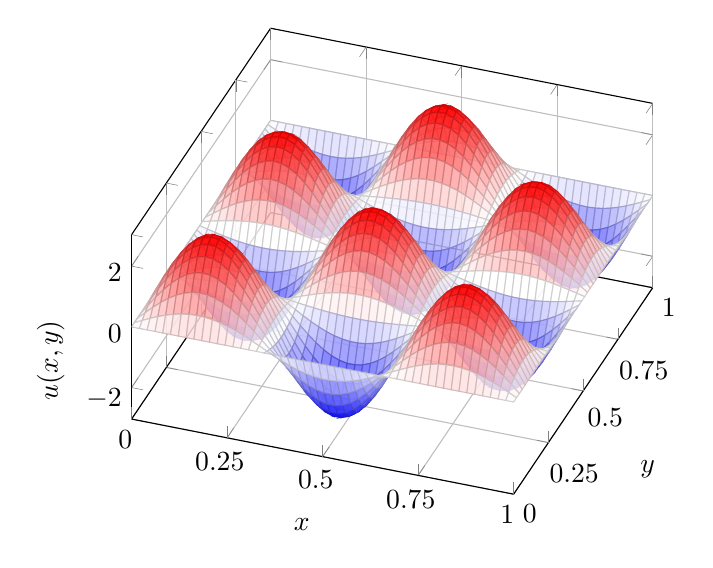
\begin{tikzpicture}
    \pgfplotsset{colormap={redblue}{rgb=(0,0,1) rgb=(1,1,1) rgb=(1,0,0)}}
\begin{axis}[
	width=8.2cm, height=7.5cm,
%	zmin=0.0,zmax=0.13,
	xlabel=$x$, xtick distance=0.25,
	ylabel=$y$, ytick distance=0.25,
  samples=50,
%	ztick={0,#2, 1/8}, zticklabels={0,#2, 1/8},
%	scaled taicks=false,
  grid,
	% title={Test},
  zlabel={$u(x, y)$},
  colormap name=redblue,
	view={20}{50},
]
	\addplot3 [
		surf,
		domain=0:1,
    opacity=0.85,%shader=interp,
	] {sin(deg(3 * pi * x)) * sin(deg(4 * pi * y)) / pi^2 * (3^2 + 4^2)};
\end{axis}
  \end{tikzpicture}
  \caption{The solution $u(x, y) = \sin(m \pi x)\sin(n \pi y) / ((n\pi)^2 + (m\pi)^22), ~m=3, n=4$ to the manufactured Poisson equation with inhomogenity $f=\sin(m \pi x)\sin(n \pi y)$.}
  \label{fig:pde:order_solution}
\end{figure}

\begin{figure}[tb]
  \centering \begin{tikzpicture}
  \begin{loglogaxis}[
      title={Demonstration of order of the five and nine point stencil.},
      xlabel={$N = N_x = N_y$},
      ylabel={Absolute error, $\lVert u - v \rVert_\infty$},
      legend pos=south west,
    ]
    \addplot[mark=none, dashed] table[x={Ns}, y={five_roof}] {PDE/order.dat};
    \addlegendentry{$C h^2$};
    \addplot[mark=none] table[x={Ns}, y={nine_roof}] {PDE/order.dat};
    \addlegendentry{$C h^4$};

    \addplot table[x={Ns}, y={five}] {PDE/order.dat};
    \addlegendentry{Five point};

    \addplot table[x={Ns}, y={nine}] {PDE/order.dat};
    \addlegendentry{Nine point};
  \end{loglogaxis}
\end{tikzpicture}

  \caption{Relative error for the clamped Biharmonic equation on $[0,1]^2$ using the five and nine point stencil.
    Also shown are $h^2$ and $h^4$, which are the expected convergence rates of the five and nine point stencil respectively.
    First axis shows $N$, the number of internal discretization points in one direction, so that the total number of grid points is $N^2$.
    Solution was found for the manufactured problem $f=\sin(m \pi x)\sin(n\pi y), ~m = 3, n=4$.
  }
  \label{fig:pde:order}
\end{figure}


\subsection{Solving the Biharmonic equation}
\label{sec:pde:solving}
We will now solve \eqref{eq:PDE} numerically on a manufactured problem.
Let
$$
u(x, y) =
\left(
\sin \pi x
\sin \pi y
\right)^4
e^{-(x-0.5)^2 - (y-0.5)^2}.
$$
The inhomogenity $f$ is simply found by calculating $\nabla^4 u$.
The result, which was found using a computer algebra system, is somewhat lengthy, and therefore only included as an appendix for the sake of readability.



According to equation \eqref{eq:PDE-poisson} we split the equation into a system of poisson equations by introducing a new function $g$:
\begin{align*}
  \begin{split}
    \nabla^2g &= f,\\
    \nabla^2u &= g,\\
    g = u &= 0,\quad \text{ on } \partial \Omega.
  \end{split}
\end{align*}
It is now simply a matter of applying the described fast poisson solver sequentially for the two equations.

The numerical solution is shown in figure \ref{fig:pde:bvp}.
In figure \ref{fig:pde:bvp_convergence} a convergence plot as a function of the degrees of freedom is shown, and the computation time is shown in figure \ref{fig:pde:bvp_time}.


\begin{figure}[tb]
  \centering
  \begin{tikzpicture}
    \pgfplotsset{colormap={redblue}{rgb=(0,0,1) rgb=(1,1,1) rgb=(1,0,0)}}
    \begin{axis}[
	      width=8.2cm, height=7.5cm,
        %	zmin=0.0,zmax=0.13,
	      xlabel=$x$, xtick distance=0.25,
	      ylabel=$y$, ytick distance=0.25,
 %       samples=50,
        %	ztick={0,#2, 1/8}, zticklabels={0,#2, 1/8},
        %	scaled taicks=false,
        %	grid,
	      % title={Test},
        zlabel={$u(x, y)$},
        mesh/ordering=x varies,
        mesh/cols=256,
        mesh/rows=256,
%        colormap name=redblue,
	      view={20}{50},
      ]
	    \addplot3 [
		    surf,
        point meta=explicit,
	    ] table[meta=U]{./PDE/biharmonic_solution_256.dat};
    \end{axis}
  \end{tikzpicture}
  \caption{The solution $u(x, y)$ to the Biharmonic equation. TODO:write more}
  \label{fig:pde:bvp}
\end{figure}

%% Error plot
\begin{figure}[hbp]
\centering
\begin{tikzpicture}
  \begin{loglogaxis}[
      title={},
      xlabel={$N = N_x = N_y$},
      ylabel={Absolute error, $\lVert u - v \rVert_2$},
      legend pos=south west,
    ]
    \addplot table[x={N}, y={error}] {PDE/error_bvp.dat};
    \addlegendentry{Nine point};
  \end{loglogaxis}
\end{tikzpicture}
\caption{
  The absolute error of the numerical solution to the clamped Biharmonic equation, using the manufactured solution $\left(
\sin \pi x
\sin \pi y
\right)^4
e^{-(x-0.5)^2 - (y-0.5)^2}$.
  TODO: Could add five point for comparison?}
\label{fig:pde:bvp_convergence}
\end{figure}

%% Computation time plot
\begin{figure}[hbp]
\centering
\begin{tikzpicture}
  \begin{loglogaxis}[
      title={},
      xlabel={$N = N_x = N_y$},
      ylabel={Computation time [s]},
      legend pos=north west,
    ]
    \addplot table[x={N}, y={FPS}] {PDE/comp_bvp_both.dat};
    \addlegendentry{Fast Poisson Solver};

    \addplot table[x={N}, y={NO_FPS}] {PDE/comp_bvp_both.dat};
    \addlegendentry{Scipy Sparse Solver};
  \end{loglogaxis}
\end{tikzpicture}
\caption{
  TODO: write
}
\label{fig:pde:bvp_time}
\end{figure}


%% For creating convergence plots and to use as a test on the validity of our approach, we will also find the analytical solution to the equation.
%% The function $f$ fulfills $f(x,y) = 0$ for $(x,y)\in \partial\Omega$, and we may thus use the analytical results derived in section \ref{sec:pde:anal}.
%% Fourier transforming $f$ results in 
%% \begin{equation*}
%% 	\hat{f}_{mn} =
%% 	\left[ 2 \integral{\sin^4(\pi x) \sin(m \pi x) e^{-(x-1/2)^2}}{x}{0}{1}\right]
%% 	\left[ 2 \integral{\sin^4(\pi y) \sin(n \pi y) e^{-(y-1/2)^2}}{y}{0}{1}\right].
%% \end{equation*}
%% The integrals do have analytical solutions, but they are not easy to compute.
%% We have computed them with the SAGE CAS suite.
%% Below is an easy-to-copy expression for the first bracket $ = I(m)$ in the equation above.
%% Then $\hat{f}_{mn} = I(m) \, I(n)$.
%% %% Old wrong result
%% %% >>> I(m) = 48*(pi^9*m^5*e^2 - 20*(pi^9*e^2 + 2*pi^7*e^2)*m^3 - (pi^9*m^5 - 20*(pi^9 + 2*pi^7)*m^3 + 16*(4*pi^9 + 15*pi^7 + 5*pi^5)*m)*(-1)^m + 16*(4*pi^9*e^2 + 15*pi^7*e^2 + 5*pi^5*e^2)*m)/(pi^10*m^10*e^3 - 20*(2*pi^10*e^3 - pi^8*e^3)*m^8 + 16384*pi^8*e^3 + 16*(33*pi^10*e^3 - 20*pi^8*e^3 + 10*pi^6*e^3)*m^6 + 40960*pi^6*e^3 - 320*(8*pi^10*e^3 - 7*pi^8*e^3 - 2*pi^4*e^3)*m^4 + 33792*pi^4*e^3 + 256*(16*pi^10*e^3 + 35*pi^6*e^3 + 20*pi^4*e^3 + 5*pi^2*e^3)*m^2 + 10240*pi^2*e^3 + 1024*e^3)
%% \begin{lstlisting}
%% I(m) = 2 * integral(sin(pi*x)^4*sin(m*pi*x)*exp(-(x-1/2)^2), x, 0, 1)
%% >> 1/16*sqrt(pi)*(erf(-2*I*pi + 1/2*I*pi*m + 1/2)*e^(4*pi^2*m)*sin(1/2*pi*m) - erf(-2*I*pi + 1/2*I*pi*m - 1/2)*e^(4*pi^2*m)*sin(1/2*pi*m) + 4*erf(-I*pi + 1/2*I*pi*m + 1/2)*e^(3*pi^2*m + 3*pi^2)*sin(1/2*pi*m) - 4*erf(-I*pi + 1/2*I*pi*m - 1/2)*e^(3*pi^2*m + 3*pi^2)*sin(1/2*pi*m) + 6*erf(1/2*I*pi*m + 1/2)*e^(2*pi^2*m + 4*pi^2)*sin(1/2*pi*m) - 6*erf(1/2*I*pi*m - 1/2)*e^(2*pi^2*m + 4*pi^2)*sin(1/2*pi*m) + 4*erf(I*pi + 1/2*I*pi*m + 1/2)*e^(pi^2*m + 3*pi^2)*sin(1/2*pi*m) - 4*erf(I*pi + 1/2*I*pi*m - 1/2)*e^(pi^2*m + 3*pi^2)*sin(1/2*pi*m) + erf(2*I*pi + 1/2*I*pi*m + 1/2)*sin(1/2*pi*m) - erf(2*I*pi + 1/2*I*pi*m - 1/2)*sin(1/2*pi*m))*e^(-1/4*pi^2*m^2 - 2*pi^2*m - 4*pi^2)

%% Funnet f etter ny endring:
%% 4*(6*pi^4*e^(x + y)*sin(pi*x)^4 - 8*(4*pi*y^3*e^x*sin(pi*x)^4 - 6*pi*y^2*e^x*sin(pi*x)^4 - 6*pi^3*e^x*sin(pi*x)^2 + 4*(2*pi^2*x - pi^2)*cos(pi*x)*e^x*sin(pi*x)^3 + (3*pi + 16*pi^3 - 2*pi*x^2 + 2*pi*x)*e^x*sin(pi*x)^4 + 4*(3*pi^3*e^x*sin(pi*x)^2 - 2*(2*pi^2*x - pi^2)*cos(pi*x)*e^x*sin(pi*x)^3 - (pi + 8*pi^3 - pi*x^2 + pi*x)*e^x*sin(pi*x)^4)*y)*cos(pi*y)*e^y*sin(pi*y)^3 + (4*y^4*e^x*sin(pi*x)^4 - 8*y^3*e^x*sin(pi*x)^4 - 8*(3*pi + 4*pi*x^3 + 16*pi^3 - 6*pi*x^2 - 4*(pi + 8*pi^3)*x)*cos(pi*x)*e^x*sin(pi*x)^3 + (256*pi^4 + 4*x^4 - 8*(16*pi^2 + 1)*x^2 - 8*x^3 + 64*pi^2 + 4*(32*pi^2 + 3)*x + 1)*e^x*sin(pi*x)^4 + 6*pi^4*e^x - 24*(2*pi^3*x - pi^3)*cos(pi*x)*e^x*sin(pi*x) - 12*(13*pi^4 - 6*pi^2*x^2 + 6*pi^2*x + 2*pi^2)*e^x*sin(pi*x)^2 + 8*(2*(pi - 2*pi*x)*cos(pi*x)*e^x*sin(pi*x)^3 - (16*pi^2 - x^2 + x + 1)*e^x*sin(pi*x)^4 + 3*pi^2*e^x*sin(pi*x)^2)*y^2 - 4*(4*(pi - 2*pi*x)*cos(pi*x)*e^x*sin(pi*x)^3 - (32*pi^2 - 2*x^2 + 2*x + 3)*e^x*sin(pi*x)^4 + 6*pi^2*e^x*sin(pi*x)^2)*y)*e^y*sin(pi*y)^4 - 24*(2*pi^3*y*e^x*sin(pi*x)^4 - pi^3*e^x*sin(pi*x)^4)*cos(pi*y)*e^y*sin(pi*y) + 12*(6*pi^2*y^2*e^x*sin(pi*x)^4 - 6*pi^2*y*e^x*sin(pi*x)^4 + 6*pi^4*e^x*sin(pi*x)^2 - 4*(2*pi^3*x - pi^3)*cos(pi*x)*e^x*sin(pi*x)^3 - (13*pi^4 - 2*pi^2*x^2 + 2*pi^2*x + 2*pi^2)*e^x*sin(pi*x)^4)*e^y*sin(pi*y)^2)*e^(-x^2 - y^2 - 1/2)
%% \end{lstlisting}
%% Something something sine transform.




%% \begin{figure}
%% \begin{tikzpicture}
%% \begin{axis}[
%% 	xmin=0, xmax=27,
%% 	declare function={
%% 		myfunc(\m)=48*(pi^9*(\m)^5*e^2 - 20*(pi^9*e^2 + 2*pi^7*e^2)*(\m)^3 - (pi^9*(\m)^5 - 20*(pi^9 + 2*pi^7)*(\m)^3 + 16*(4*pi^9 + 15*pi^7 + 5*pi^5)*(\m))*(-1)^(\m) + 16*(4*pi^9*e^2 + 15*pi^7*e^2 + 5*pi^5*e^2)*(\m))/(pi^10*(\m)^10*e^3 - 20*(2*pi^10*e^3 - pi^8*e^3)*(\m)^8 + 16384*pi^8*e^3 + 16*(33*pi^10*e^3 - 20*pi^8*e^3 + 10*pi^6*e^3)*(\m)^6 + 40960*pi^6*e^3 - 320*(8*pi^10*e^3 - 7*pi^8*e^3 - 2*pi^4*e^3)*(\m)^4 + 33792*pi^4*e^3 + 256*(16*pi^10*e^3 + 35*pi^6*e^3 + 20*pi^4*e^3 + 5*pi^2*e^3)*(\m)^2 + 10240*pi^2*e^3 + 1024*e^3);
%% 	},
%% 	xtick={1,6,...,26},
%% 	minor x tick num=4,
%% 	xlabel=$m$, title={$I(m)$},
%% ]
%% \addplot [domain=1:26, samples=26, mark=*] {myfunc(x)};
%% \addplot [domain=0:27, samples=2, dashed] {0};
%% \end{axis}
%% \end{tikzpicture}
%% \end{figure}



\newpage
\appendix
\section{The inhomogenity \texorpdfstring{$f$}{f}}
In section \ref{sec:pde:solving} the Fast Poisson Solver was applied on the manufactured solution $u$.
The inhomogenity $f = \nabla^4 u$ was ommited in the text, due to it being lengthy.
It is here shown in full, together with the code used to find it, using the Sage CAS.
\begin{lstlisting}
sage: u(x, y) = (sin(pi * x) * sin(pi * y))^4 * e^(-(x-1/2)^2 - (y-1/2)^2)
sage: (u.diff(x, 4) + u.diff(y, 4) + 2 * u.diff(x, 2).diff(y, 2)).full_simplify()
>> 4*(6*pi^4*e^(x + y)*sin(pi*x)^4 - 8*(4*pi*y^3*e^x*sin(pi*x)^4 - 6*pi*y^2*e^x*sin(pi*x)^4 - 6*pi^3*e^x*sin(pi*x)^2 + 4*(2*pi^2*x - pi^2)*cos(pi*x)*e^x*sin(pi*x)^3 + (3*pi + 16*pi^3 - 2*pi*x^2 + 2*pi*x)*e^x*sin(pi*x)^4 + 4*(3*pi^3*e^x*sin(pi*x)^2 - 2*(2*pi^2*x - pi^2)*cos(pi*x)*e^x*sin(pi*x)^3 - (pi + 8*pi^3 - pi*x^2 + pi*x)*e^x*sin(pi*x)^4)*y)*cos(pi*y)*e^y*sin(pi*y)^3 + (4*y^4*e^x*sin(pi*x)^4 - 8*y^3*e^x*sin(pi*x)^4 - 8*(3*pi + 4*pi*x^3 + 16*pi^3 - 6*pi*x^2 - 4*(pi + 8*pi^3)*x)*cos(pi*x)*e^x*sin(pi*x)^3 + (256*pi^4 + 4*x^4 - 8*(16*pi^2 + 1)*x^2 - 8*x^3 + 64*pi^2 + 4*(32*pi^2 + 3)*x + 1)*e^x*sin(pi*x)^4 + 6*pi^4*e^x - 24*(2*pi^3*x - pi^3)*cos(pi*x)*e^x*sin(pi*x) - 12*(13*pi^4 - 6*pi^2*x^2 + 6*pi^2*x + 2*pi^2)*e^x*sin(pi*x)^2 + 8*(2*(pi - 2*pi*x)*cos(pi*x)*e^x*sin(pi*x)^3 - (16*pi^2 - x^2 + x + 1)*e^x*sin(pi*x)^4 + 3*pi^2*e^x*sin(pi*x)^2)*y^2 - 4*(4*(pi - 2*pi*x)*cos(pi*x)*e^x*sin(pi*x)^3 - (32*pi^2 - 2*x^2 + 2*x + 3)*e^x*sin(pi*x)^4 + 6*pi^2*e^x*sin(pi*x)^2)*y)*e^y*sin(pi*y)^4 - 24*(2*pi^3*y*e^x*sin(pi*x)^4 - pi^3*e^x*sin(pi*x)^4)*cos(pi*y)*e^y*sin(pi*y) + 12*(6*pi^2*y^2*e^x*sin(pi*x)^4 - 6*pi^2*y*e^x*sin(pi*x)^4 + 6*pi^4*e^x*sin(pi*x)^2 - 4*(2*pi^3*x - pi^3)*cos(pi*x)*e^x*sin(pi*x)^3 - (13*pi^4 - 2*pi^2*x^2 + 2*pi^2*x + 2*pi^2)*e^x*sin(pi*x)^4)*e^y*sin(pi*y)^2)*e^(-x^2 - y^2 - 1/2)
\end{lstlisting}
\clearpage
\printbibliography
%% \begin{thebibliography}{99}
%% \bibitem{owren}
%% Brynjulf Owren:
%% \textit{TMA4212 Numerical solution of partial differential equations with finite difference methods}
%% (2017)
%% [\url{http://www.math.ntnu.no/emner/TMA4212/2020v/notes/master.pdf}]

%% \end{thebibliography}

\end{document}
